\documentclass[french]{llncs}

\usepackage[english, french]{babel}
\usepackage[utf8]{inputenc}

\usepackage{graphicx}

\usepackage{listings}
\usepackage{subfig}
\usepackage{hyperref}
\usepackage{dirtytalk}

\usepackage{color}
\usepackage{caption}
\usepackage{algorithm}
\usepackage{algorithmic}
\renewcommand{\algorithmicrequire}{\textbf{Entrée:}}
\renewcommand{\algorithmicensure}{\textbf{Sortie:}}
\renewcommand{\algorithmiccomment}[1]{\{#1\}}
\renewcommand{\algorithmicend}{\textbf{fin}}
\renewcommand{\algorithmicif}{\textbf{si}}
\renewcommand{\algorithmicthen}{\textbf{alors}}
\renewcommand{\algorithmicelse}{\textbf{sinon}}
\renewcommand{\algorithmicfor}{\textbf{pour}}
\renewcommand{\algorithmicforall}{\textbf{pour tout}}
\renewcommand{\algorithmicdo}{\textbf{faire}}
\renewcommand{\algorithmicwhile}{\textbf{tant que}}
\renewcommand{\algorithmicelsif}{\algorithmicelse\ \algorithmicif}
\renewcommand{\algorithmicendif}{\algorithmicend\ \algorithmicif}
\renewcommand{\algorithmicendfor}{\algorithmicend\ \algorithmicfor}

%-----------------------------------------
\title{Apprentissage statistique pour la prédiction des interactions chromosomiques}

%\subtitle{\vspace{.5cm}Rapport de Master}

\author{ Océane \textsc{Cassan} 
\newline{}{Encadrée par Laurent \textsc{Bréhélin}, Charles-Henri \textsc{Lecellier}, Sophie \textsc{Lèbre}}}


\institute{Université Claude Bernard Lyon 1\\
INSA de Lyon, France}


\lstset{ 
    basicstyle=\small,
    captionpos=b  % sets the caption-position to bottom
}


\providecommand{\motcles}[1]{\textbf{Mots-clés:} #1}

\pagestyle{headings} 
%-----------------------------------------

\begin{document}

\clearpage\thispagestyle{empty}\addtocounter{page}{-1} 

    \renewcommand{\thelstlisting}{\arabic{lstlisting}}

    \maketitle

    \selectlanguage{french}
    \begin{abstract} L'identité d'une cellule est déterminée par le profil d'expression de ses gènes. Les repliements dynamiques de la molécule d'ADN à l'intérieur du noyau permettent de mettre en contact différentes régions régulatrices, afin de moduler la fixation des protéines initiant la transcription des gènes. Les mécanismes régissant ces contacts ne sont encore que partiellement compris, ainsi que les nombreux paramètres biologiques les gouvernant. L'influence de l'environnement de l'ADN est très décrite dans la littérature, contrairement à l'influence de la séquence directement. L'objectif de ce stage est donc de déterminer si les séquences a elles seules permettent de prédire les contacts entre les régions régulatrices, dans un contexte d'apprentissage automatique. La construction de jeux de données adaptés basés sur des expériences biologiques est proposée, ainsi qu'une méthode d'extraction de \textit{features} par segmentation des séquences. Différents types de modèles de classification supervisée sont entraînés sur ces jeux de données, et comparés. Les résultats montrent que les variables liées à la séquence ne portent pas toute l'information recherchée. De plus, l'environnement des régions régulatrices semble plus informatif que les séquences elles mêmes pour prédire leur mise en contact.
\\
         \\
        
         \motcles{ 
        Interactions chromosomiques, apprentissage automatique, génomique, bioinformatique, extraction de features
    }
    \end{abstract}

   
    \clearpage\thispagestyle{empty}\addtocounter{page}{-1} 
    
    
    \selectlanguage{english}
    \begin{abstract}
        Abstract in english.
        
         \begin{keywords}
        keywords
    \end{keywords}
    \end{abstract}

\clearpage
   

%-----------------------------------------


\clearpage\thispagestyle{empty}\addtocounter{page}{-1} 

\section*{Remerciements}

Il me tient à coeur de commencer en remerciant toutes les personnes ayant fait de ce stage une expérience riche.

Tout d'abord, je remercie sincèrement Laurent Bréhélin pour la qualité de son encadrement et sa grande disponibilité. Il s'est montré d'une aide incontestable pour guider notre projet à chacune de ses étapes. 

Je souhaite également remercier Charles-Henri Lecellier pour les précieux conseils offerts sur le cadre biologique du stage, ainsi que pour son intérêt communicatif envers les subtilités de la génétique.


Merci à Sophie Lèbre, dont les apports en statistique ont éclairé plus d'un aspect de mon travail. Je me réjouis de notre collaboration plus étroite dans un futur proche.

Je suis très reconnaissante à Christophe Menichelli pour avoir partagé avec moi son excellent travail de thèse, et m'avoir permis de prendre part à son extension. 

Enfin, je remercie Raphaël Romero, dont le travail sur des thématiques proches a permis un échange fructueux d'informations.

Les fréquentes réunions avec ces personnes ont permis un suivi précis, personnalisé, aussi apprécié qu'utile au projet. Je leur souhaite à tous une très bonne continuation au sein de l'équipe, dans laquelle évoluer pendant 5 mois fut un réel plaisir.


Enfin, je remercie Sergio Peigner, m'ayant encadrée du côté de l'INSA, et Sam Meyer qui a accepté d'être le second membre de mon jury.


\vfill

\hrule
\vfill
\begin{center}
\say{Nature composes some of her loveliest poems for the microscope and the telescope.}
Theodore Roszak, Where the Wasteland Ends, 1972
\end{center}
\vfill 
\hrule 
\vfill


\clearpage
\clearpage\thispagestyle{empty}\addtocounter{page}{-1} 
\tableofcontents

\clearpage


\newpage


\section{Contexte} \label{intro}

\subsection{Cadre biologique}

Toutes les cellules de notre organisme possèdent le même code génétique. L'existence de différents tissus ou types cellulaires est permise par une grande diversité des profils d'expression des gènes dans chacune de nos cellules. Les gènes dits actifs, ou exprimés, définissent fondamentalement une cellule au travers des protéines qui la composent, de ses fonctions métaboliques, ou de ses capacités d'adaptation à l'environnement.

Le processus biologique qui module l'expression des gènes est la transcription.
Il s'agit d'un mécanisme au cours duquel un complexe protéique, l'ARN polymérase, vient se fixer à la molécule d'ADN, l'ouvre, et synthétise une ARN messager contenant la séquence d'un gène précis. Cet ARN messager sera ensuite exporté à l'extérieur du noyau et traduit en protéine pour ensuite exercer sa fonction dans la cellule.

Le recrutement de la polymérase se fait via les facteurs de transcription, des protéines venant se lier à des régions situées en amont d'un gène, des régions dites promotrices. Les régions promotrices, ou promoteurs, ne codent pas d'information comme le font les gènes, mais permettent de réguler leur transcription via leur séquence et leur accessibilité en accueillant les protéines initiant la transcription.
Des régions régulatrices plus distantes des gènes, appelées les enhancers, peuvent également être impliquées dans leur régulation. Dans ce cas, leur contact avec un promoteur via des repliements de la molécule d'ADN s'avère indispensable à la transcription, et permet de créer des patterns d'expression génétique plus complexes, flexibles et robustes. Chez les vertébrés, ces régions distantes sont connues pour interagir de manière dynamique avec les promoteurs pour constituer des profils d'expression tissu-spécifiques \cite{robson_regulatory_2019}. 

Ces interactions longue-distance sont rendues possibles par les repliements tri-dimensionnels de la chromatine. La chromatine est composée de l'ADN enroulé autour de protéines, appelées histones, qui lui confèrent sa structure et définissent son degré de compaction. Des forces physiques antagonistes, entre répulsion et attraction moléculaires \cite{robson_regulatory_2019}, régissent la spatialisation de la chromatine. Ainsi, les enhancers peuvent s'affranchir de distances chromosomiques de l'ordre du Mégabase pour communiquer leur information régulatrice à un promoteur, comme illustré en Figure \ref{fig/regulation}. Ces contacts se produisent le plus souvent au sein d'un même chromosome, mais des rapprochements inter-chromosomiques sont également observés. D'une manière plus large, le repliement de la chromatine met en contact de nombreuses régions régulatrices actives simultanément dans des compartiments fonctionnels appelés les TADS : Topologically Associated Domains.

\begin{figure}[h]
\begin{center}
 	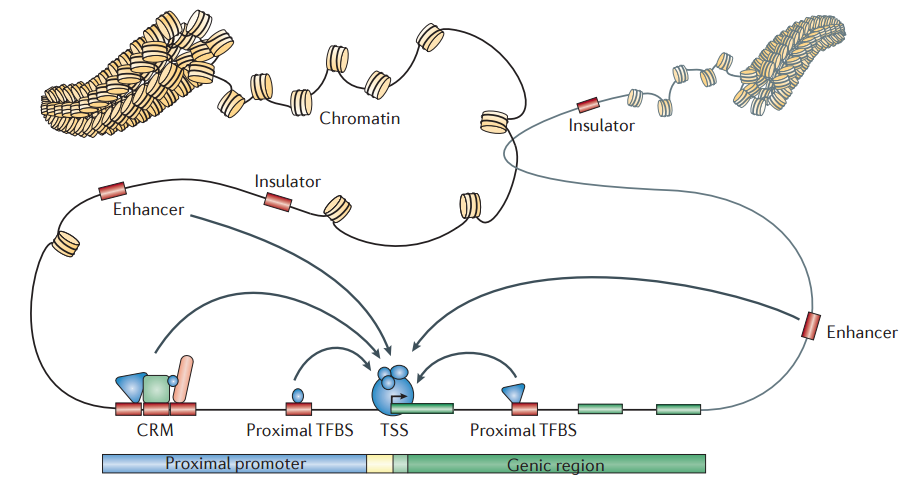
\includegraphics[width=0.85\linewidth]{Images/regulation.png}
 \caption{Vue schématique d'un gène et de ses régions régulatrices, issu d'un fragment de chromatine déroulée. Le promoteur est en bleu et ses enhancers en rouge. Le contact se fait précisément au niveau du TSS (Transcription Starting Site), et amorce la transcription de la région génique en aval.\cite{lenhard_metazoan_2012}} \label{fig/regulation}
\end{center}
\end{figure}


Parmi ce concert de mouvements gouvernés par les voies métaboliques et adaptatives de la cellule et admettant une certaine stochasticité, identifier quels enhancers régulent quels gènes dans un type cellulaire particulier demeure une question difficile. Beaucoup de travaux publiés tendent à montrer que des variables épi-génétiques, c'est à dire liées à l'environnement de l'ADN, à sa conformation, ou à des modifications chimiques apportées aux histones peuvent être informatives, mais peu s'intéressent à la séquence nucléotidique directement. L'objectif de ce stage est de savoir s'il est possible de prédire l'interaction entre deux régions chromosomiques impliquées dans la régulation en se basant sur leur séquence uniquement.

\subsection{Sources de données pour les interactions chromosomiques} \label{section:donnees}


Des consortiums internationaux fournissent aujourd'hui une cartographie assez complète de l'ensemble
des enhancers et promoteurs du génome humain. Par exemple le consortium FANTOM (Fonctional ANonTation Of the Mammalian genome) créé en 2000 a pu les répertorier en utilisant une méthode basée sur la mesure des ARN d'expression (e-ARN) de ces régions. En effet, lors de la transcription des gènes, les enhancers et le promoteurs génèrent transcrits. Ces courts transcripts "capés" sont capturés par la technique CAGE (Cap Analysis Gene Expression). Ces e-ARN ont des caractéristiques différentes chez les enhancers et les promoteurs, ce qui permet de les différencier. Après alignement, leur localisation sur les chromosomes est répertoriée \cite{the_fantom_consortium_atlas_2014} \cite{the_fantom_consortium_and_the_riken_pmi_and_clst_dgt_promoter-level_2014}. La base de données FANTOM contient environ 40 000 enhancers, et 95\% des promoteurs des gènes annotés comme codant pour des protéines à ce jour. Ce travail a été fait sur plus de 500 types cellulaires différents chez l'homme, et l'atlas constitué a été utilisé tout au long de ce stage pour définir et nommer les régions chromatiniennes étudiées. La nomenclature utilisée pour un promoteur sera par exemple \texttt{chr10:7890..7925,+}, signifiant qu'il est situé sur le chromosome 10, commence à la base 7890 et se termine à la base 7925. Après la virgule, le signe + ou - informe sur le brin d'ADN, direct ou complémentaire, sur lequel se situe le promoteur. Pour un enhancer, les identifiants seront de la forme \texttt{chr12:43690..43877}. La signification reste la même, à la différence d'absence d'information sur le sens du brin, car les e-ARN CAGE caractéristiques des enhancers sont bidirectionnels.

Une fois la liste des régions régulatrices établie, la question est d'obtenir l'information de leur rapprochement dans l'espace. Pour cela, on distingue différentes approches.

\paragraph{Les techniques expérimentales de détection de contacts}

Des techniques d'identification des contacts chromatiniens appelés Chromosome Conformation Capture Analysis (3C) permettent de constituer de telles bases de données. Parmi elles, notre attention s'est portée sur deux types de capture : 
\begin{itemize}
    \item Les expériences de Hi-C. Les portions génomiques mises en contact sont liées par des \textit{linkers}, des petites séquences d'ADN se chaînant à tout fragment d'ADN proche de lui. Les linkers se lient aux régions régulatrices en contact, puis s'en suit une phase de dégradation de l'ADN par une enzyme de restriction, qui détruit la molécule d'ADN non liée. On obtient, à l'issu de la coupe des \textit{linkers}, des paires de portions d'ADN issues de deux fragments spatialement proches dans le noyau. 
    
    \item Les expériences de ChIA-PET. Ces expériences sont très proches des expériences de Hi-C. La technique de Hi-C capture les interactions se produisant sur tout le génome sans restrictions, tandis que les données de ChIA-PET filtrent les contacts faisant intervenir une protéine d'intérêt. Ainsi, nous obtenons les paires de régions en contact médié par une certaine protéine, par exemple un facteur de transcription précis, ou l'ARN polymérase.
    
\end{itemize}

Ces techniques garantissent des jeux de données riches et suffisamment résolutifs pour traiter notre problématique. Elles restent néanmoins
lourdes et difficiles à mettre en place sur de nombreux types cellulaires.
C'est ce qui a motivé d'autres méthodes de constitution de paires de régions chromosomiques, généralisables à un grand nombre de types cellulaires.

\paragraph{L'association de régions suivant une corrélation d'expression}

 Dans la publication de leur Atlas des enhancers \cite{the_fantom_consortium_atlas_2014}, le consortium FANTOM réalise des associations entre enhancers et promoteurs, en utilisant les mesures d'expression obtenues par la méthode CAGE dans leurs nombreux types cellulaires. Une valeur d'expression est un nombre de \textit{reads} d'e-ARNs séquencés pour cette région dans le type cellulaire considéré.
 
 Cette démarche de constitution de paires part du postulat qu'un enhancer qui régule un promoteur doit avoir un profil d'expression similaire à celui du promoteur dans l'ensemble des tissus analysés. 
 Pour chaque couple enhancer-promoteur de leurs atlas, les corrélations sont calculées deux à deux entre les profils d'expression. Chaque mesure de corrélation fournit un p-valeur renseignant sur la significativité de la corrélation, et donc de l'appariement de l'enhancer et du promoteur considérés. Cette procédure impliquant des tests multiples, une correction a été appliquée dans le calcul des p-values, la méthode False Discovery Rate. Cette méthode permet de contrôler le nombre de faux positifs dans l'ensemble des tests. Au final, 340150 paires enhancer-promoteur significatives sont identifiées.

Bien qu'elle ne nécessite pas d'expérimentations coûteuses comme celles des 3C (outre la technique CAGE), cette méthode perd l'information de l'appariement enhancer-promoteur dans un type cellulaire précis. En effet, les corrélations sont calculées sur tous les types cellulaires, donnant en résultat un score d'appariement global.

\subsection{Formalisation du problème d'apprentissage statistique}

Les jeux de données précédemment décrits constituent la matière première de l'apprentissage supervisé que nous souhaitons mettre en place. Ces jeux de données permettent d'entraîner un modèle prédictif avec une \textit{ground truth} pour un ensemble fourni de régions chromosomiques, mais également de tester ce modèle sur un ensemble réservé à l'évaluation. En effet, une propriété fondamentale de l'apprentissage statistique est la capacité de distinguer des patterns sur un ensemble d'apprentissage, pour ensuite les généraliser à des données inconnues.

Les modèles d'apprentissage automatiques envisagés doivent permettre, pour une paire de régions chromosomiques en entrée, de prédire si ces régions vont se retrouver en contact dans l'espace du noyau cellulaire ou non. Étant donnée la nature tissu-spécifique de ces interactions, notamment entre enhancer et promoteurs, l'objectif est de construire les modèles de manière spécifique à un type cellulaire. Différentes variables en \textit{input} de ces modèles caractérisant la séquence des régions à prédire seront explorées. De plus, plusieurs méthodes de \textit{machine learning} seront étudiées afin de répondre au mieux à la problématique traitée.


\subsection{État de l'art}

Les interactions entre régions régulatrices ont déjà été étudiées dans la littérature, et il existe plusieurs travaux visant à les prédire. En sont présentés ici quelques uns, ayant nourri la réflexion préalable à ce projet.

Certaines méthodes publiées ne font pas appel à du \textit{machine learning}. Par exemple, ABC model \cite{fulco_activity-by-contact_2019} définit un score comme le produit de l'expression de l'enhancer par la fréquence des contacts entre l'enhancer et le promoteur dans des types cellulaires connus. Cette fréquence des contacts est donnée par des expériences 3C, et l'expression par les \textit{peaks} CAGE pour de nombreux types cellulaires. Plus ce score est élevé, plus il est probable que l'enhancer et le promoteur soient en contact. Cependant, cette méthode reste simple et ne permet pas de retranscrire toutes les subtilités des données. 

Un article souvent cité pour l'utilisation de modèles de \textit{machine learning} dans la prédiction des interactions enhancer-gènes est l'article présentant le modèle TargetFinder \cite{whalen_enhancerpromoter_2016}. Les variables de leurs modèles sont liées à des mesures d'ouverture de la chromatine, à la méthylation \footnote{La méthylation est une altération chimique des bases de l'ADN, via l'ajout d'un groupement méthyle. Elle est connue pour jouer un rôle clé dans la régulation des gènes.} de l'ADN, à l'expression, à la fixation de facteurs de transcription et de protéines structurales, ou à la modification des histones. Ces variables sont observées en dynamique dans les types cellulaires, et traduisent leur paysage épi-génétique, sans s'intéresser directement à la séquence. Les modèles de \textit{machine learning} proposés prennent en entrée l'ensemble de ces \textit{features} pour chaque élément d'une paire (enhancer, promoteur, et fenêtre les séparant), pour faire une prédiction.
Parmi les modèles testés, la méthode ensembliste à base de \textit{Boosted Trees} a été plus performante qu'un \textit{linear SVM} ou qu'un arbre de décision seul. La méthode de quantification de l'importance des variables est celle implémentée dans ce le package \texttt{scikit-learn}, par Hastie et Al \cite{hastie2005elements}. Les auteurs parviennent à discriminer les paires interagissant, labelisées grâce à des données de Hi-C, et atteignent une performance de 83\% sur la moyenne des types cellulaires. Ce chiffre est cependant à nuancer car un travail \cite{xi_local_2018} a été publié en 2018 afin de corriger une erreur de cette publication. En effet, les modèles présentés sont basés sur des variables structurelles et épi-génétiques décrivant les enhancers, les promoteurs, et la portion d'ADN les séparant. Lorsque N enhancers consécutifs interagissent avec le même promoteur, sont formées N paires distinctes. Or, ces paires partagent des caractéristiques au niveau du promoteur et de la région les séparant, appelée la fenêtre. 
Si deux paires se chevauchent, même si elles font intervenir des promoteurs ou enhancers différents, elles peuvent partager certaines \textit{features} via leur fenêtre. Si le jeu de test comporte des paires partageant des \textit{features} avec des paires rencontrées lors de l'apprentissage, les capacités de généralisation se voient faussées par une sur-spécificité au jeu d'entraînement. Les auteurs de cet article correctif suggèrent de classer les paires par position chromosomique afin que les paires contenant des éléments en commun se retrouvent uniquement dans le jeu d'apprentissage ou de test, et non dans les deux simultanément comme le ferait une cross-validation aléatoire. Les nouvelles valeurs de score f1 utilisées pour quantifier la performance de la classification de TargetFinder après cette correction sont montrées en annexe 1, figure \ref{fig/correction_biais}, et attestent que les prédictions ne sont en réalité pas meilleures que le hasard.
 Ce phénomène de biais de \textit{features} partagées sera donc pris en compte dans l'élaboration des jeux d'apprentissage et de test du projet.



D'autres méthodes, comme celle intitulée RIPPLE \cite{roy_predictive_2015}, visent à prédire les interactions dans tous les types cellulaires.
Celle-ci entraîne d'abord des \textit{classifiers} spécifiques aux types cellulaires un utilisant les marques des histones, les sites de fixation de facteurs de transcription, et les niveaux d'e-ARN. Les variables pour l'enhancer et le promoteur sont ensuite combinées en en faisant le produit, l'addition, ou la corrélation. Ces modèles permettent la sélection de variables, et les variables sélectionnées sont utilisées pour nourrir un \textit{Random Forest} plus général, prédisant les interactions enhancer-promoteur de manière globale, quel que soit le type cellulaire.

A l'inverse, les auteurs de la procédure JEME \cite{cao_reconstruction_2017} commencent par combiner l'information commune à tous les types cellulaires. Le principe est de sélectionner des variables informatives sur l'ensemble des types cellulaires grâce à des régressions logistiques pénalisées, puis de les utiliser dans des \textit{Random Forests} propres au type cellulaire. Encore une fois, les variables utilisées sont des mesures d'accessibilité de l'ADN, les \textit{peaks} d'e-RNA, et la distance entre l'enhancer et le promoteur.

Le \textit{deep learning} a très récemment fait son apparition dans la litérature concernant les interactions enhancer-promoteur. Les auteurs de la méthode SPEID \cite{singh_predicting_2018} ont été les premiers a s'intéresser à la séquence uniquement pour prédire ces contacts. Leur modèle est un réseau de neurones composé de plusieurs couches de convolutions, suivies d'un réseau récurrent Long Short Term Memory (LSTM). Cette approche permet l'extraction de \textit{features} par convolution des séquences fournies en entrée, (celles de l'enhancer et du promoteur), puis combine ces \textit{features} dans une architecture récurrente, adaptée à la nature séquences séquentielle des données.
Cette méthode semble permettre la prédiction de telles interactions, mais ne laisse pas la liberté de choisir et analyser les variables biologiques informatives. En effet, les convolutions et \textit{max-pooling} qui en découlent sont peu interprêtables.

Les auteurs de cette méthode ont également, un an auparavant, développé une approche qui s'avère la plus proche de nos objectifs : PEP \cite{yang2017exploiting}. Son module PEP-Motif a pour principe d'extraire des scores d'occurrence de motifs (courtes séquences d'ADN) connus pour recruter des facteurs de transcription, et de les utiliser comme variables prédictives d'un modèle de Gradient Tree Boosting. Les résultats présentés sont très encourageants, mais s'appuient cependant sur le même jeu de données que TargetFinder, lequel présentais un biais de surévaluation de ses performances. La validité de ces très bons résultats est donc remise en question par les travaux présentés en référence \cite{xi_local_2018}.

Au terme de cet état de l'art, il est envisagé de s'inspirer des modèles rencontrés, tels que la régression logistique, les méthodes ensemblistes, ou le \textit{deep learning}, mais en utilisant des variables d'une nature différente. Contrairement à la grande majorité des articles rencontrés, nous souhaitons utiliser des variables prédictives uniquement liées aux séquences, et non aux signaux fonctionnels et structuraux de liés à molécule d'ADN. Nous cherchons à construire des modèles plus intelligibles que les modèles de \textit{deep learning} ne permettant pas l'étude de variables biologiques, et à vérifier les résultats des quelques méthodes (\cite{yang2017exploiting} et \cite{singh_predicting_2018}) suggérant que la séquence à elle seule peut être informative.

\section{Méthodes}

\subsection{Caractérisation d'une séquence d'ADN}

Différentes variables peuvent être considérées lorsque nous cherchons à caractériser une séquence d'acides nucléiques. L'ADN se compose d'un alphabet de 4 nucléotides, A, C, G et T, respectivement Adénine, Cytosine, Guanine et Thymine. Les proportions de ces bases et leur arrangement en motifs précis sont connus pour être liés à la nature des régions génomiques ainsi qu'à leur fonction régulatrice \cite{vandel_probing_2019} \cite{bessiere_probing_2018}.
La taille des séquences considérées variera suivant les tests réalisés. Elle est, dans les modèles initiaux, de 1000 paires de bases (bp), centrée sur le milieu de la région régulatrice.

\paragraph{La composition en nucléotides : }
 La proportion des nucléotides, également appelées bases, constitue une première information à capter. Au delà d'une seule base, l'information la fréquence de plusieurs bases consécutives est à considérer, comme la fréquence de dinucléotides, tri-nucléotides ou de quadri-nucléotides. Plus généralement, la notion de k-mer se réfère à un mot de $k$ nucléotides. Au total, à l'instar des variables utilisées dans la référence \cite{vandel_probing_2019}, 12 variables de composition nucléotidique seront utilisées dans les modèles, : les taux de AT et CG, représentant la fréquence des nucléotides A et T sur les deux brins d'ADN, et de C et G, ainsi que les taux de 10 dinucléotides. Les détails sur le choix de ces 10 2-mers sur les 16 possibles avec un alphabet de 4 lettres sont présentés en annexe 2.


\paragraph{Les motifs dénommés PWM : }

Les facteurs de transcription reconnaissent des k-mers particuliers, motifs nécessaires à leur fixation. Il existe environ 1600 facteurs de transcription connus chez l'homme. Les expériences de Chip-Seq permettent d'établir quels sont les motifs sur lesquels se fixent préférentiellement chaque facteur. Lors d'une telle d'expérience, les séquences fixées par le facteur étudié sont protégées d'une immunoprécipitation de la molécule l'ADN, puis séquencées. Cela permet d'aboutir à un k-mer consensus, car les motifs de fixation ne sont pas stricts, mais autorisent une certaine variabilité. Ces consensus représentent les probabilités de trouver les 4 nucléotides à chaque position du k-mer qui maximisent l'affinité de la séquence avec le facteur de transcription considéré.
Il existe des bases de données de ces motifs appelés PWM (Position Weight Matrix), comme la base Jaspar \cite{sandelin_jaspar:_2004} qui en répertorie 662. sur les 1600 environ connus chez l'homme. Il est possible de les visualiser sous forme de logos comme montré en figure \ref{fig/logo_pwm}.

\begin{figure}[h]
\begin{center}
 	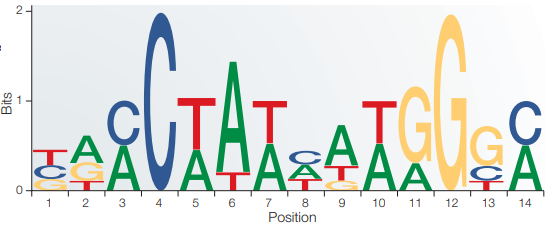
\includegraphics[width=0.6\linewidth]{Images/LOGO.PNG}
 \caption{Exemple de motif PWM. La taille des lettres des nucléotides varie suivant à la probabilité de le trouver en position donnée par l'abscisse. } \label{fig/logo_pwm}
\end{center}
\end{figure}

Des logiciels développés et optimisés pour la recherche d'occurrences sont ensuite utilisés pour repérer ces motifs dans un set de séquences d'intérêt. Un score PWM est obtenu en calculant l'adéquation entre les k-mers de la séquence et les différentes versions des motifs PWM connus. À l'issue de ce processus, il est possible d'attribuer aux séquence désirées un score pour chaque facteur de transcription, représentant les chances de présence d'un motif pour lequel ce facteur a une forte affinité. Ces scores constitueront un second type de variables explorées au cours de ce stage.

\subsection{Modèles de classification}\label{section:models}

Pour quantifier le niveau d'information porté par les séquences pour prédire les interactions chromosomiques, des modèles de classification de nature différente ont été envisagés et comparés.

\paragraph{La régression logistique pénalisée}

La régression linéaire est une méthode statistique permettant de trouver une relation linéaire entre une variable réponse Y et un ensemble de variables prédictives X.
Son écriture matricielle est la suivante :
\begin{equation}
Y = X\beta + \epsilon,
\end{equation}
avec $\beta$ le vecteur de coefficients, et $\epsilon$ l'erreur aléatoire, dite résiduelle. Lorsque l'on ajuste un modèle linéaire, le vecteur de coefficients est estimé de manière minimiser l'erreur quadratique $\sum_{i = 1}^{n}(y_i - \hat{y}_i)^2$, avec $y_i$ la valeur à prédire, et $\hat{y}_i$ la valeur prédite par le modèle.


Les coefficients estimés permettent de réaliser des prédictions sur la variable réponse. Cependant, cela reste insuffisant pour réaliser une sélection de variables expliquant significativement la réponse. Cette question est particulièrement importante quand la dimensionalité de l'espace des variables est grande, nécessitant d'identifier les variables les plus informatives.

Pour cette raison, il est possible d'appliquer une méthode pénalisant la régression classique. Lors de l'estimation des coefficients, une contrainte supplémentaire est ajoutée sur le vecteur de coefficients, dont la norme ne doit pas excéder une certaine constante $\lambda$, appelée pénalité ou paramètre de tuning. Suivant la norme choisie, on parle de différentes méthode de régularisation. S'il s'agit de la norme 1, c'est à dire la somme en valeur absolue des coefficients, on parle de la Méthode du Lasso, pour Least Absolute Shrinkage and Selection Operator. Lorsque la norme 2 est employée, c'est à dire la somme du carré des coefficients on parle de la pénalisation Ridge. Une combinaison de ces deux normes conduit à la régularisation Elastic Net. Plus le paramètre de tuning est stringeant, plus le modèle est contraint et doit diminuer la valeur des coefficients qui lui sont le moins utiles pour minimiser l'erreur. La régularisation que nous avons choisie est la méthode du Lasso, en raison de sa capacité à fixer la valeur des coefficients les moins informatifs à 0, comme illustré sur la figure \ref{fig/lasso}.

\begin{figure}[h]
\begin{center}
 	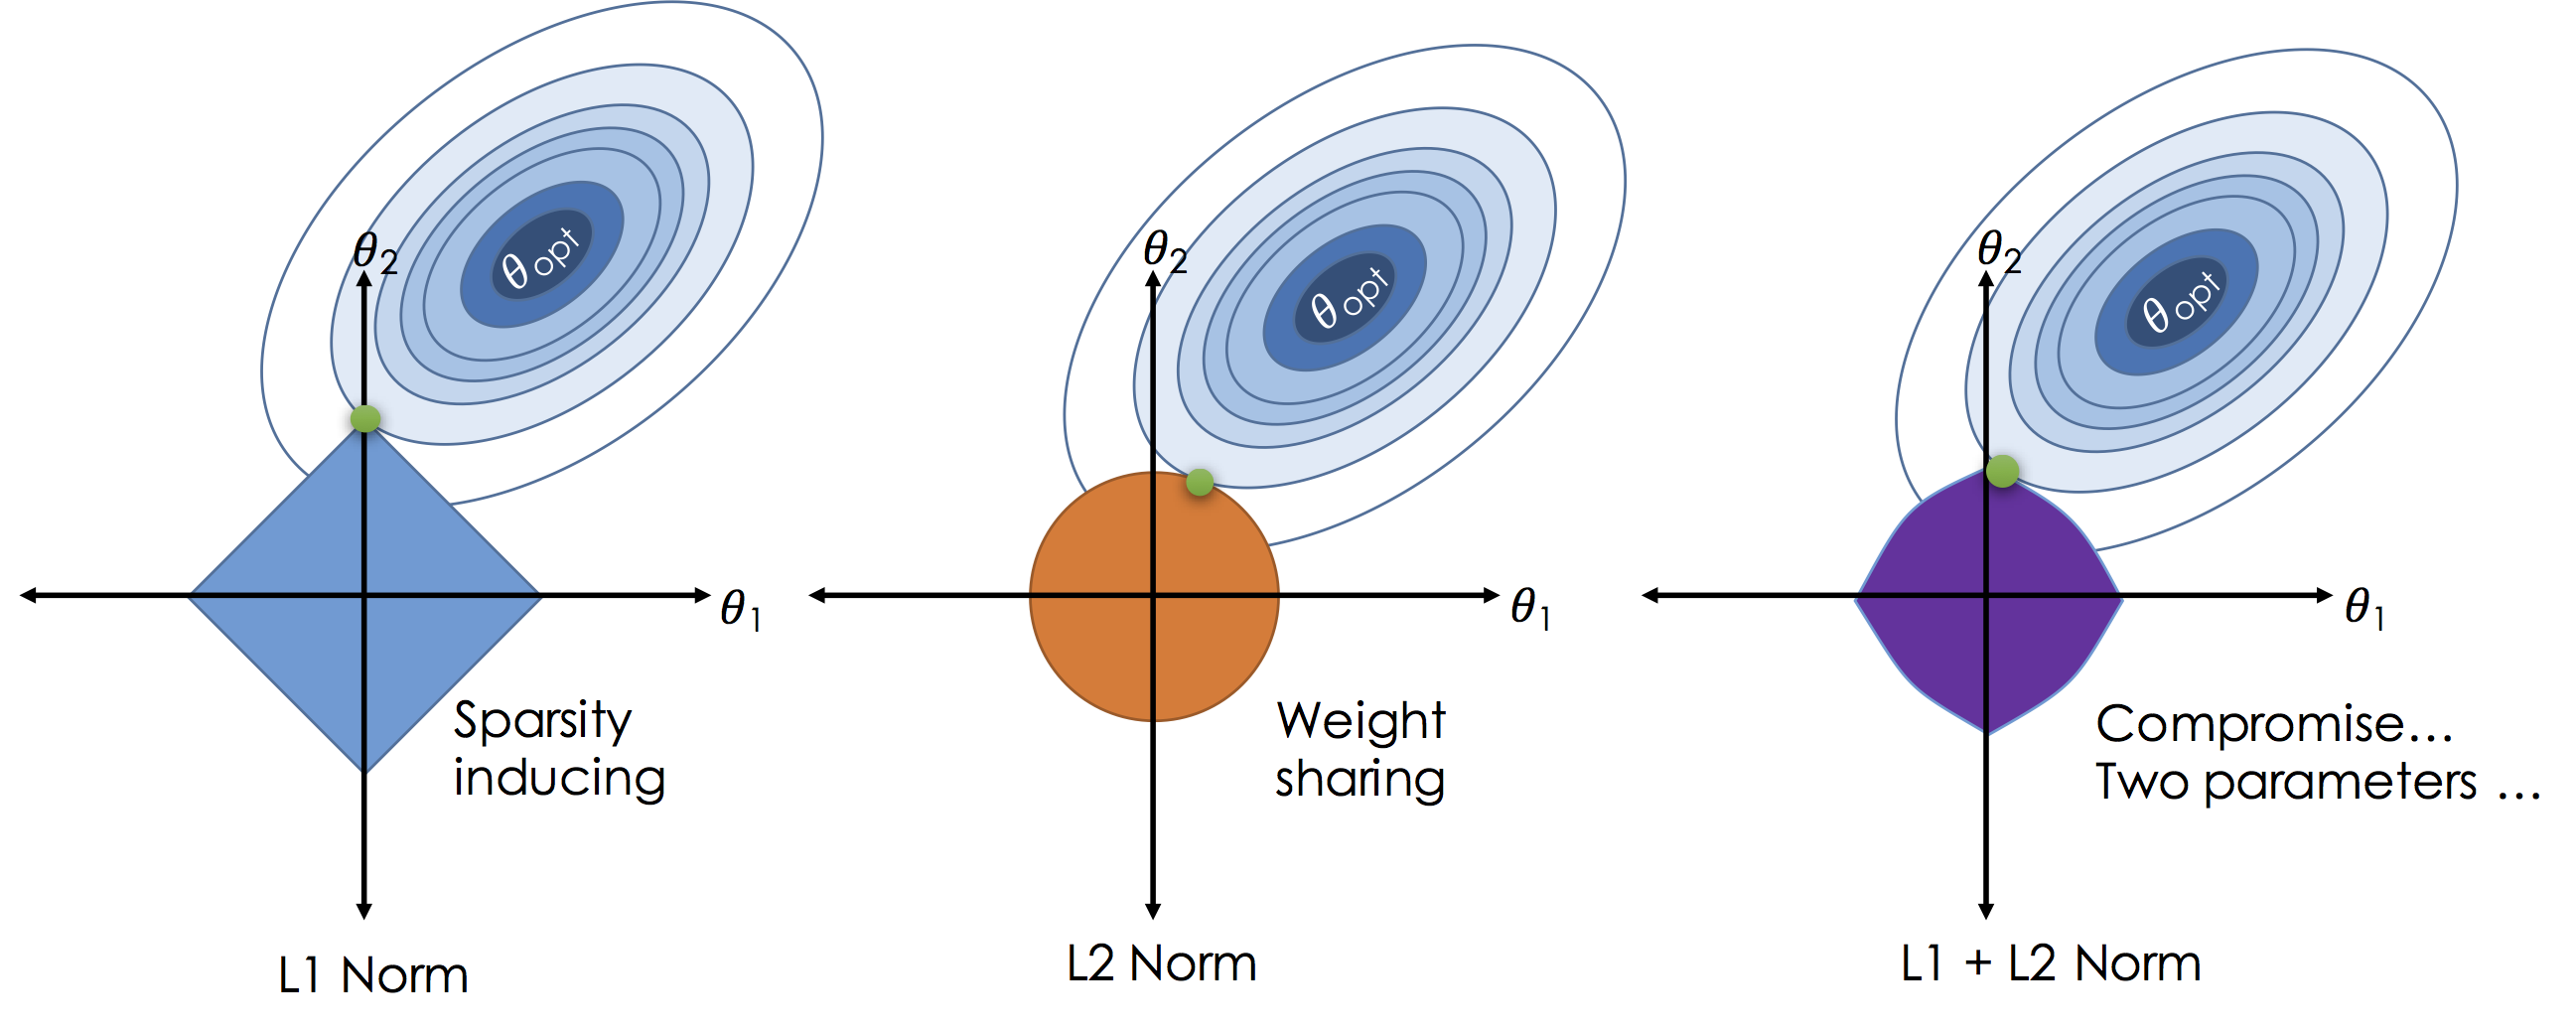
\includegraphics[width=1\linewidth]{Images/Lasso-Ridge.png}
 \caption{Représentation des différents types de régularisation dans une espace de coefficients à deux dimensions. La zone $\theta_{\mathrm{opt}}$ représente les valeurs de coefficients minimisant l'erreur prédictive du modèle. Lorsque l'on ajoute une régularisation, les coefficients estimés seront à l'intersection entre cette zone optimale et la boule de la norme mathématique associée à la pénalité choisie. La norme L1, pour le Lasso, crée une boule carrée, favorisant le placement des coefficients sur l'un des axes du plan, le mettant à 0. La méthode Ridge utilisant la norme 2 minimise ces coefficients sans les fixer à 0, et Elastic Net trouve un compromis entre les deux. Source : The Biais Variancec Readeoff and regularization, slides by Joseph E. Gonzales.} \label{fig/lasso}
\end{center}
\end{figure}
La fonction à optimiser lors de l'estimation des coefficients se formalise donc

\begin{equation}
\sum_{i = 1}^{n}(y_i - \hat{y}_i)^2 + \lambda \sum_{j=1}^p|\beta_j| = \sum_{i = 1}^{n}(y_i - \sum_{j=1}^p\beta_jX_{ij})^2 + \lambda \sum_{j=1}^p|\beta_j|,
\end{equation}

avec n le nombre d'observations utilisées pour ajuster le modèle, et p le nombre de variables explicatrices. L'argmin de cette fonction, c'est à dire le vecteur de coefficients $\beta$, est obtenu par des méthodes d'optimisation telles que la descente de gradient.

Pour choisir la valeur de $\lambda$, une plage de valeurs est généralement testée. Des modèles sont ajustés sur un jeu d'entraînement, pour différentes valeurs de $\lambda$, et testés pour chaque valeur de $\lambda$ sur un jeu de test indépendant. La valeur choisie est celle qui minimise l'erreur sur le jeu de test. Lorsque le jeu de données n'est pas suffisamment grand, il vaut mieux procéder par k-fold cross validation. Cette technique consiste à découper le jeu de données en k partitions. k-1 partitions sont utilisées pour entrainer le modèle, et la dernière permet de le tester. Cette démarche est répétée k fois, de manière à ce que chaque partition ait servi une fois de test. Pour chaque jeu de test, on choisit la valeur optimale de $\lambda$. En regardant les valeurs de $\lambda$ sur les k jeux de test, nous avons une valeur de $\lambda$ qui maximise les performances calculée sur l'ensemble du jeu d'apprentissage.


Une régression linéaire pénalisée réalise des prédictions quantitatives. Dans notre contexte, un modèle de classification permettant de prédire une sortie binaire (interaction ou non des régions chromosomiques présentées) est requis. C'est donc la régression logistique du modèle linéaire généralisé que nous avons utilisée. Plutôt que d'estimer la valeur Y directement, le logarithme de l'odds d'interaction, également nommée fonction logit, est approximé par une combinaison linéaire des variables. La régression logistique se formalise ainsi :
\begin{equation}
\mathrm{logit}(p_{\mathrm{interaction}}) = \mathrm{ln}\large(\frac{p_{\mathrm{interaction}}}{1-p_\mathrm{interaction}}\large) = X\beta + \epsilon,
\end{equation}
 avec $p_\mathrm{interaction}$ la probabilité de contact entre deux régions régulatrices.
 
Le principe de régularisation peut tout aussi bien y être appliqué afin de sélectionner les variables les plus importantes. 
Des implémentations de régressions logistiques pénalisées incluant la validation croisée sont disponibles en R dans le package \texttt{glmnet} \cite{friedman_regularization_2010}, ou en python dans la librarie \texttt{scikt learn} \cite{scikit-learn}. C'est la version du langage R qui a été majoritairement utilisée au cours du stage, avec la fonction la fonction \texttt{cv.glmnet} et 10 folds pour la validation croisée.

\paragraph{Les Random Forests}

Un arbre de décision est une structure prédictive construite à partir de grandes quantités de données. Les variables permettant de discriminer au mieux la variable réponse sont repérées à partir de mesures d'entropie ou de l'indice de Gini suivant la nature de l'arbre. Chaque noeud représente une condition sur une variable. Plus une variable explique la séparation de la réponse entre les classes à prédire, plus elle est placée en haut de l'arbre.  Au bas de l'arbre, se trouvent les feuilles représentant la décision du modèle. Il s'agit de modèles très interprétables, car ils peuvent être vus comme une série de requêtes et de tests à propos des données aboutissant à une prédiction. Ils sont introduis pour la première fois en 2001, avec la publication de Breiman et Al. \cite{breiman2001random}.

Un arbre de décision seul peut fournir des résultats satisfaisants, mais est connu pour souffrir de problèmes de stabilité et d'\textit{overfitting}. La combinaison de plusieurs arbres permet une performance accrue dans la classification, tout en réduisant considérablement les risques d'\textit{overfitting}. Le principe de cette méthode dite ensembliste est de créer un ensemble d'arbres qui, pris séparément, sont des \textit{weak learners}\footnote{Un \textit{weak learner} est un modèle de \textit{machine learning} effectuant des prédictions meilleures que le hasard, même légèrement.}, mais dont les décisions collectives sont significativement meilleures.

Pour parvenir à un meilleur pouvoir de classification, les arbres de la foret doivent pouvoir rendre des décisions complémentaires, dues à des différences structurelles. Deux techniques sont employées dans cette optique :

\begin{itemize}
    \item Le \textit{bootstrapping} : les différents arbres sont entraînés sur des jeux de données échantillonnés avec remise dans le jeu de données initial. Ainsi, certaines observations seront dupliquées, d'autres seront absentes suivant les jeux d'entraînement, causant des choix de variables discriminantes différents entre les arbres.
    
    \item À chaque noeud, l'arbre de décision ne pourra utiliser qu'un nombre réduit de variables tirées parmi la liste totale des variables.
\end{itemize}

Ces opérations associées à l'\textit{averaging} des prédictions de tous les arbres, permettent de réduire le bruit présent dans les données.
Il est également possible d'accéder assez rapidement à l'importance des variables utilisées pour la classification d'un modèle de \textit{Random Forests}. L'une des méthodes principales repose sur les \textit{Out Of the Bag examples}, les éléments ayant été écartés de l'apprentissage lors du \textit{bootstrapping}. Ces éléments n'ayant pas participé à l'ajustement des modèles peuvent être utilisés pour tester l'importance des variables. Cette importance est donnée par la différence d'\textit{accuracy} entre le modèle sur les données de test, et le jeu de test dans lequel la variable d'intérêt a été randomisée. Cette perte de performance pour une variable et calculée pour tous les arbres, permet de quantifier en moyenne l'apport de cette variable dans les capacités de classification d'une Random Forest.
C'est cette technique qui est utilisée par les \texttt{RandomForestClassifier} de \texttt{scikit-learn}. 

Les \textit{Random Forests} utilisés dans le cadre du stage utilisent le critère de Gini pour quantifier la pureté d'un noeud, et contiennent 200 individus. Cette valeur de 200 individus a été obtenue au terme d'une GridSerachCV optimisant le critère d'AUC\footnote{Ce critère est décrit en section \ref{section:auc}} du modèle.

\paragraph{Le Stochastic Gradient Boosting}

L'intuition du \textit{boosting} est de corriger de manière itérative des modèles prédictifs, en accordant une importance plus forte aux éléments les moins bien estimés. Cette méthode peut être appliquée à des arbres de décisions et entre, tout comme les \textit{Random Forests}, dans la catégorie des méthodes ensemblistes. La différence est que les différents prédicteurs ne sont pas entraînés de manière indépendante, mais séquentielle.

Le \textit{Gradient Boosting} correspond au fait d'ajuster un nouveau modèle, à chaque itération de l'algorithme, aux résidus du modèle précédent. En effet, si les prédictions ne sont pas satisfaisantes, on peut supposer qu'un \textit{pattern} reste à trouver dans l'erreur résiduelle du modèle. Soit un modèle de l'itération $m$ $F_m(x)$ attribuant des prédictions à un vecteur variable $x$. Les pseudo-résidus sont calculés comme la dérivée négative de l'erreur par rapport aux prédictions du modèle. Ces résidus servent de jeu d'entraînement pour le modèle suivant que l'on désigne par $h_{m+1}(x)$. La valeur de $\gamma$ est trouvée de manière à minimiser l'erreur du nouveau modèle $F_{m+1}(x) = F_m(x) + \gamma h_{m+1}(x)$, modèle qui est ensuite ajouté à l'ensemble des modèles et servira de base pour l'itération suivante. 
La décision du modèle de \textit{Gradient Boosting} sera la moyenne des $M$ modèles ainsi obtenus.



Le \textit{Stochastic Gradient Boosting } ajoute une composante aléatoire à l'algorithme précédant. Le principe est de n'utiliser qu'une fraction du jeu de données total tirée aléatoirement pour entraîner les modèles $F_m(x)$ au début de chaque itération.
Cet ajout permet un gain en robustesse par rapport au \textit{Gradient Boosting}. Cependant, les méthodes additives telles que le \textit{Gradient Boosting} sont connues pour être un peu plus sensibles à l'\textit{overfitting}\footnote{L'\textit{overfitting} correspond à un sur-spécificité d'un modèle par rapport à son jeu d'apprentissage, et par conséquent à une incapacité de généralisation correcte sur de nouvelles données.} que les méthodes indépendantes comme les \textit{Random Forests}.

\paragraph{Perceptron multi-couches} Un réseau de neurones est une technique de \textit{deep learning} usuellement utilisée en classification supervisée. Un réseau se compose d'unités élémentaires excitables, les neurones. Disposées en couches et reliées entre elles, en l'occurrence de manière \textit{fully connected}, cette structure permet l'approximation de fonctions. Chaque connexion est caractérisée par un poids, et ces poids sont appris de manière à minimiser l'erreur entre les prédictions du réseau et ce qui est attendu. Un apprentissage se compose de deux phases, itérativement répétées. Tout d'abord, la propagation de l'activité est faite à partir d'une donnée présentée au réseau. La prédiction du réseau est comparée à la sortie attendue, fournissant une valeur d'erreur. Une rétro-propagation de cette erreur est alors effectuée, corrigeant les poids de manière proportionnelle à la dérivée partielle de l'erreur par rapport à chaque poids. Un réseau de neurones a de multiples hyper-paramètres, comme le nombre de couches, le nombre de neurones par couches, la fonction d'activation des neurones, ou la fonction d'erreur, aussi dite \textit{optimizer}.
Un perceptron multicouche est utilisé dans la seconde partie du projet, dans un optique d'exploration et de validation simple. Ne représentant pas un axe principal de ce stage, l'accent ne sera donc pas mis sur sa paramétrisation ni sur la recherche d'une structure de réseau plus complexe. Le perceptron utilisé est le perceptron \texttt{MLP} du package sci-kit learn. Il est utilisé avec la fonction d'activation RELU, l'\textit{optimizer} Adam et 100 neurones par couches.

\subsection{Évaluation des performances d'un modèle}\label{section:auc}

Lors de l'évaluation d'un modèle de classification, il est d'usage de comparer le vecteur de prédictions obtenu sur un jeu de test aux labels connus, aussi dits \textit{ground truth}. La comparaison de ces deux vecteurs peut être faite de différentes manières afin de renseigner sur les performances du modèle. Une approche naïve est de calculer la fréquence des éléments correctement classifiés, donnant une mesure de l'\textit{accuracy}. Il est également possible de compter le nombre de vrais-faux négatifs et positifs, donnant des mesures de précision et de rappel pour ces classes.

Nous avons choisi l'utilisation du critère d'Area Under Curve (AUC) pour quantifier différemment des capacités prédictives. L'AUC mesure l'aire sous la courbe ROC. Cette courbe est obtenue en traçant les taux de vrais positifs en fonction des taux de faux positifs pour différentes valeurs seuils binarisant les prédictions quantitatives\footnote{Cela correspond à tracer la sensibilité du modèle en fonction de un moins sa spécificité. D'autres courbes existent et font apparaître la précision en fonction du rappel : leur AUC permet de définir un critère de performance de classification encore différent.}. Un modèle donnant une AUC à 0.5 est comparable à une classification au hasard, et plus l'AUC se rapproche de 1, plus le modèle est performant.
Alors que l'accuracy pourrait être haute sur un modèle prédisant une valeur constante sur un jeu de données déséquilibré, l'AUC s'affranchit de se problème en se concentrant sur le pouvoir séparateur d'un modèle par rapport à des prédiction aléatoires. Un exemple de courbe ROC et de l'AUC associée sont visibles en figure\ref{fig:rocs_fantom_ep_nucl}.

\subsection{Prédiction des interactions enhancer-gènes}\label{section:methdoes_ep}

Au cours de la première partie du stage, nous avons souhaité prédire les contacts enhancer-gène de manière tissu spécifique, en se basant à la fois sur la composition nucléotidique des régions chromosomiques et sur leurs scores PWM. Dans un premier temps la question de la construction d'un jeu d'apprentissage équilibré se pose.

\subsubsection{Sélection des exemples positifs et négatifs} \label{section:chia-pet}

Dans les jeux de données mentionnés en section \ref{section:donnees}, les exemples de paires enhancer-promoteur en interaction sont clairement identifiables. Cependant, dans un contexte d'apprentissage automatique, il nous faut également choisir un ensemble de paires (dites négatives) qui ne sont pas en contact. Il s'agit du \textit{background}, les paires contre lesquelles nous souhaitons faire ressortir un signal. Le choix du \textit{background} est crucial car il ne fera pas apparaître les mêmes informations prédictives suivant sa composition. Suivant l nature des données les exemple négatifs ont été construits différemment.


\paragraph{Paires pré-constituées par le consortium FANTOM :}

Dans leur article \cite{the_fantom_consortium_atlas_2014}, les auteurs de l'atlas des promoteurs et des enhancers du génome humain constituent des associassions enhancers-promoteurs basées sur une mesure d'expression de ces régions parmi toutes leurs librairies \footnote{Une librairie désigne un type cellulaire.}. Il en résulte un ensemble de paires valables sur un ensemble d'environ 600 types cellulaires. Or, étant donnée la tissu spécificité de l'action des enhancers, nous souhaitons créer un jeu de données par type cellulaire. Les données d'expression des enhancers et des promoteurs FANTOM sont accessibles sous format matriciel. Ces matrices contiennent la valeur d'expression de chaque promoteurs et enhancers dans chacune des librairies.

Dans une première approche, nous sommes donc partis du principe que pour un type cellulaire précis, les paires enhancers-promoteurs positives seront les paires FANTOM pré-constituées par corrélation qui ont à la fois leur enhancer et leur promoteur actifs dans ce tissu. Pour définir cette notion d'activité, nous sélectionnons les enhancers et promoteurs dont le niveau d'expression est strictement supérieur à 0. Une visualisation de ces ensembles est montrée en figure \ref{fig/paires_fantom}. Pour les paires négatives, les paires dont le promoteur est actif et dont l'enhancer est inactif ont été choisies, pour traduire le cas où un promoteur est exprimé, mais régulé par un autre enhancer. 

\begin{figure}[h]
\begin{center}
 	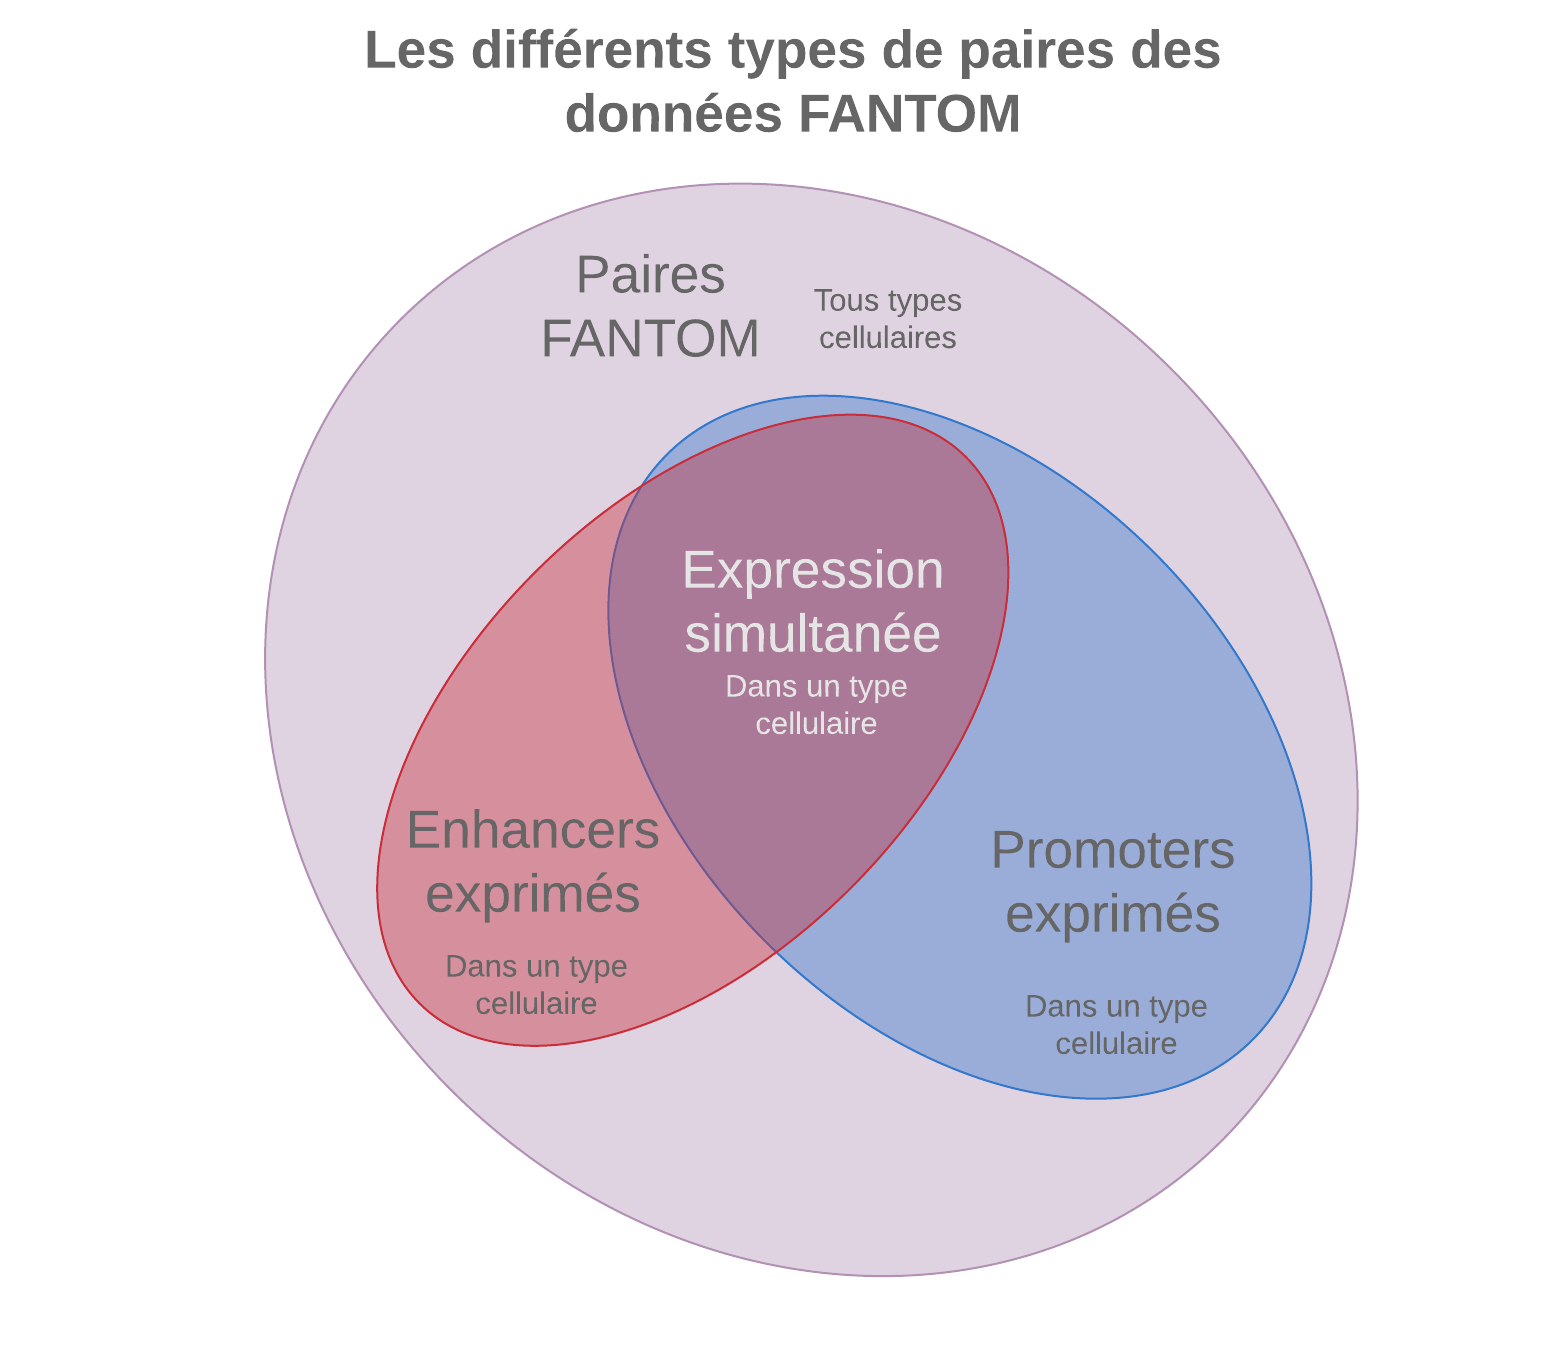
\includegraphics[width=0.7\linewidth]{Images/FANTOM_pairs.png}
 \caption{Diagramme des paires constituées par le consortium FANTOM intersectées avec les paires dont l'enhancer et/ou le promoteur sont actifs dans un type cellulaire précis.} \label{fig/paires_fantom}
\end{center}
\end{figure}

Pour éviter tout biais, il est important de contrôler l'expression des promoteurs dans la classe positive et la classe négative. En effet, les promoteurs peu exprimés risquent d'être sur-représentés dans la classe négative,ce qui introduirait un facteur de confusion dans l'étude. Au moment de constituer les paires négatives, des paires avec des mesures d'expression similaires à celles de la classe positives sont échantillonnés. Les mesures d'expression pouvant contenir des valeurs extrêmement fortes en petit nombre, c'est le logarithme de l'expression qui a été utilisé pour cet échantillonage. Cela permet de resserrer la distribution et de réduire la proportion d'\textit{outliers}, facilitant la création d'une distribution proche de celle de la classe positive.

Le problème ainsi défini revient à prédire les paires avec enhancers et promoteurs actifs, contre celles dont seul le promoteur est actif. De fait, le problème se réduit dans ce cas à un problème de classification de l'activité des enhancers. Nous avons donc imaginé une seconde problématique. Les paires positives considérées sont ici les paires FANTOM dont l'enhancer et le promoteur sont simultanément soit actifs, soit inactifs. De même, les paires négatives sont les paires dans lesquelles uniquement l'un des membres de la paire est actif. Une comparaison et une interprétation biologique de ces deux problématiques sera faite dans la section résultats. Comme précédemment, un contrôle sur l'expression est effectué afin de considérer des promoteurs ayant des activités similaires dans les deux classes.

\paragraph{Paires obtenues par Chia-Pet :}

Les données brutes d'une expérience de Chia-Pet se présentent au format bed, couramment utilisé pour stocker des coordonnées génomiques. Chaque entrée de ce fichier correspond à une région chromosomique décrite par son chromosome, son début, sa fin, et la paire de régions chromosomiques à laquelle il appartient. Ces portions d'ADN peuvent cependant se situer n'importe où dans le génome, il est donc nécessaire de les filtrer par régions régulatrices connues pour rester dans la problématique fixée. L'intersection de ces régions est donc faite avec les régions chromosomiques correspondant à celles de la base de données FANTOM.
Cette intersection est réalisée grâce à un outil fourni par la suite des \texttt{bedtools}. La fonction \texttt{intersect} permet de retourner tous les enhancers et promoteurs FANTOM qui sont couverts par les régions impliquées dans des contacts lors de l'expérience de ChIA-Pet. Une jointure est alors faite, afin de lier les enhancers et promoteurs FANTOM impliqués dans la même paire ChIA-Pet, fournissant ainsi la liste des paires enhancers-promoteurs désirées.


Ces manipulations permettent de disposer de paires positives pour l'apprentissage. Or, ces données ne portent pas directement d'informations relatives à des paires négatives, car elles contiennent uniquement les régions impliquées dans un contact.
Une méthode pour obtenir ces régions est de prendre les paires positives et de les randomiser. Un désappariement est alors effectué, pour créer des paires fictives labélisées comme n'interagissant pas. Pour se rapprocher de la nature des paires FANTOM dont la distance enhancer-promoter n'excède pas 500 kbases, ce même contrôle a été fait. Les paires shufflisées n'ont donc été gardées que si elles satisfaisaient cette contraintes, permettant des paires plus réalistes.

\subsubsection{Constitution du jeu d'apprentissage et de test}


Le jeu de données utilisé en \textit{machine learning} doit être séparé en un ensemble d'entraînement, et un ensemble de validation. Pour retranscrire au mieux les capacités de généralisation du modèle, ce jeu de validation doit être complètement indépendant du jeu d'apprentissage. En effet, si des exemples entièrement ou en partie identiques, sont retrouvés à la fois dans le jeu d'apprentissage et dans le jeu de test, le modèle ne ferait que re-mobiliser avec succès des prédictions vues lors du training, montrant des performances artificiellement hautes.

La nature des données utilisées dans ce projet rend cette problématique assez importante et plus délicate à traiter. Comme montré dans la référence \cite{xi_local_2018}, des éléments partageant certaines \textit{features}, même s'ils ne sont pas exactement identiques, peuvent conduire à une sur-estimation de l'AUC. En effet, comme les éléments à classifier sont des paires, il est possible de retrouver un même enhancer ou promoteur dans plusieurs paires. Une précaution à prendre est donc de regrouper les paires contenant un élément en commun soit dans les jeu de test, soit dans le jeu d'apprentissage uniquement. 

De la même manière, si des régions se chevauchent, il est possible que celles ci partagent des caractéristiques et biaisent l'évaluation du modèle. Comme pour les paires identiques, les paires chevauchantes seront donc contrôlées de manière à n'apparaître que lors de l'apprentissage ou de l'évaluation.

\subsubsection{Ajout de variables d'interaction}

Le jeu de données final contient autant de paires positives, c'est à dire dont l'enhancer et le promoteur sont en contact, que de paires négatives. Chaque élément d'une paire est caractérisé par sa composition nucléotidique et les scores de 662 PWM. Des jeux de données ont également été construits avec uniquement l'une de ces deux variables pour en tester l'utilité.

Les modèles considérés sont soit de nature linéaire, comme la régression logistique pénalisée, ou non linéaires, comme les méthodes ensemblistes. Il est possible que les variables de l'enhancer et du promoteur combinées de manière linéaire ne suffisent pas à expliquer l'appariement de ces régions. Contrairement aux modèles linéaires, les modèles non linéaires sont supposés pouvoir potientiellement capter des interactions intéressantes pour la prédiction. Mais il est également possible que même les modèles non linéaires aient du mal à discerner clairement cette interaction. Il pourrait alors s'avérer utile de leur fournir une variable représentant directement les deux composantes de la paire. Plusieurs fonctions on été envisagées, traduisant différentes hypothèses biologiques. Tout d'abord, le produit des variables de l'enhancer et du promoteur a été testé, le produit étant généralement utilisé dans les modèles linéaires avec interaction. Puis, pour traduire une similarité des compositions des séquences, nous avons pensé à la valeur absolue de la différence des deux variables, ou à la valeur absolue du logarithme de leur rapport. Un minimum de ces deux valeurs pourrait donner l'équivalent d'un "et" logique, un maximum représenterait "ou" logique pour les variables de compositions en nucléotides ou scores PWM. Ces variables sont nommées "variables de paire".

Au terme de ces manipulations, nous obtenons des données de travail, se présentant comme en figure \ref{fig/dataset}. Les variables de paires seront ajoutées ou non pour en tester l'influence sur les modèles.

\begin{figure}[h]
\begin{center}
 	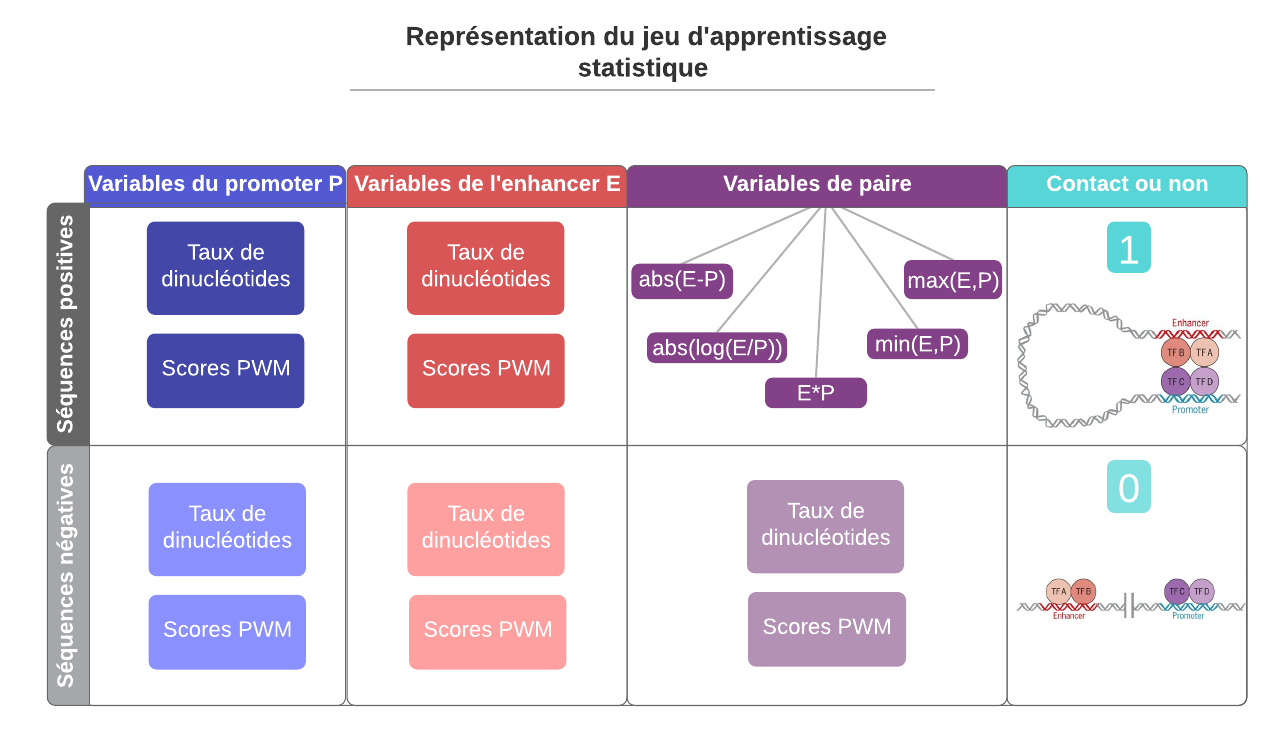
\includegraphics[width=1\linewidth]{Images_FANTOM/Dataset_interactions.png}
 \caption{Structure du jeu de données utilisé pour construire les modèles de classification. Images : Developmental enhancers and chromosome topology, Furlong et Al, 2018 \cite{furlong_developmental_2018}} \label{fig/dataset}
\end{center}
\end{figure}


\subsection{Extraction de \textit{features} par segmentation pour la prédiction des interactions promoteur-promoteur}

Les variables utilisées pour faire des prédictions dans les modèles précédents sont des variables relatives à la totalité des régions chromosomiques. Il est légitime de se demander si une extraction de \textit{features} plus précise et permettant de ne s'intéresser à des compositions de nucléotides que sur certaines zones des régions régulatrices pourrait être informatif.

Étant donnés les résultats sur les prédictions des interactions enhancers-gènes (voir section \ref{section:res_EP}), nous avons fait le choix, pour la seconde partie du stage, de réorienter les recherches. Il s'agit maintenant de prédire les interactions promoteur-promoteur, connus pour se rapprocher dans l'espace au sein des TADs, des domaines regroupant et compartimentant les gènes actifs dans le noyau.

\subsubsection{DExTER}

DExTER (Domain Exploration To Explain gene Regulation) est un algorithme développé par Christophe Menichelli au cours de sa thèse dans l'équipe MAB. Sa création a été motivée par l'intuition que dans une séquence, seulement certaines portions peuvent contenir l'information recherchée pour expliquer la régulation des gènes. L'objectif est donc d'extraire les régions dont la composition en nucléotides s'avère être la plus corrélée à une variable réponse étudiée.

Dans l'article \cite{bessiere_probing_2018}, il a été montré que la segmentation des régions promotrices s'avérait porteuse d'information pour la prédiction de la régulation de l'expression. Cette segmentation basée sur la connaissance à priori de différents régions impliquées, était cependant manuelle, et la nécessité d'un outil pouvant la réaliser de manière automatique s'est imposée.
Dans un premier temps, DExTER a servi à prédire l'expression de gènes étant donnée la séquence de leurs promoteurs, centrée autour du TSS. Ainsi, en fournissant un fichier de séquences promotrices de gènes, associé à un fichier contenant le niveau d'expression de chaque gène, DExTER est capable de fournir un ensemble de variables explicatrices de cette expression. 

DExTER entre dans la catégorie des méthodes d'extraction de \textit{features}. Une exploration des séquences est conduite de manière à déterminer quelles sont les combinaisons compositions nucléotidiques/régions de séquences les plus prédictives pour une réponse donnée, ici l'expression. Une variable, ou domaine, est donc représentée par un tuple (fréquence de k-mer, région), dénotés par la suite $D_{k,r}$. Pour décomposer une séquence, c'est la méthode de  partitionnement par treillis qui a été choisie.
Cette méthode permet de quantifier l'information de la fréquence d'un k-mer comprise entre deux intervalles de la séquence entière. La séquence entière est représentée au bas du treillis, et est découpée en un certain nombre de sous régions. Deux lignes partant respectivement de la position A et B s'intersectent en un noeud qui contient la proportion du k-mer entre les positions A et B de la séquence. Plus on monte dans le treillis, plus on se rapproche de la composition globale du k-mer dans la séquence. La figure \ref{fig/treillis} montre un exemple de cette structure.
\begin{figure}[h]
\begin{center}
 	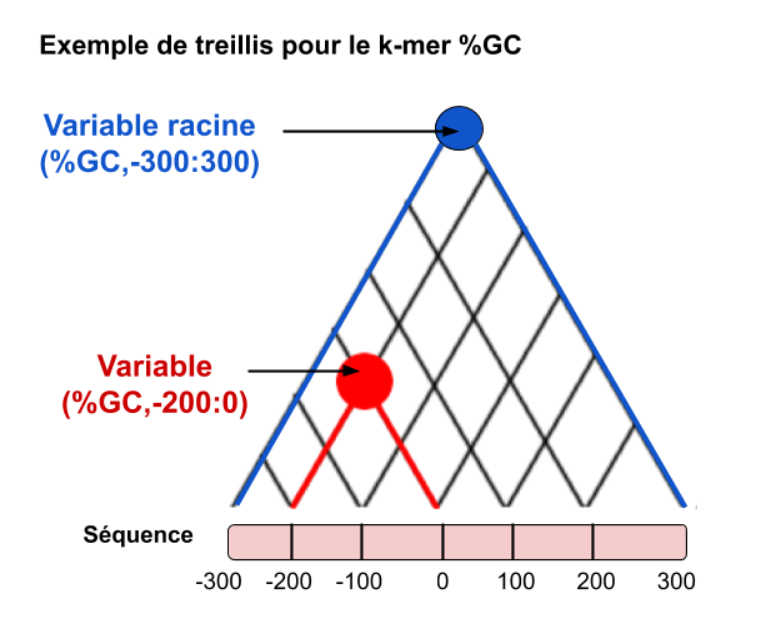
\includegraphics[width=0.5\linewidth]{Images_Dextra/Treillis.png}
 \caption{Exemple schématique d'un treillis pour le dinucléotide GC sur une séquence de 601 bases.} \label{fig/treillis}
\end{center}
\end{figure}

La procédure d'exploration consiste à parcourir les domaines notés $D_{k,r}$ représentant le k-mer $k$ sur la région $r$ des séquences totales, et d'exhiber ceux qui se montrent les plus corrélés au vecteur réponse $Y$. La liste $L$ des domaines à explorer est initialisée aux dinucléotides sur une région $r$ correspondant à l'ensemble de la séquence. Au cours de la procédure, des domaines sont ajoutés à la liste à explorer en rajoutant un nucléotide au k-mer courant, ou en ajustant la région de ce k-mer. 

On désigne par "parent" un domaine qui donne naissance à un nouveau domaine. Ce nouveau domaine peut soit être un domaine de k-mer identique à son parent, mais sur une région différente, soit un domaine de k+1 mer sur la même région que son parent. Ces phases sont alternées afin de conduire l'exploration de manière équilibrée. Lorsque l'on vient d'ajouter un nucléotide à une domaine, l'étape suivante est de re-effectuer une segmentation pour trouver la région, plus restreinte ou plus large, qui maximise la corrélation de ce k-mer avec $Y$. 

Cette mesure de corrélation est expliquée plus en détail en figure \ref{fig:treillis_global_dexter}. Pour une région donnée, il s'agit d'une corrélation de Spearman entre le vecteur de taux de k-mer sur cette région et la variable réponse, cela pour l'ensemble des séquences fournies. 

Sont retenus et ajoutés à la liste des domaines validés $L_{val}$ les domaines ayant une corrélation à Y supérieure à celle de leur parent, et qui vérifient une condition de contrôle.  Cette condition de contrôle $\mathrm{Cor}(D_{k,r}, Y) > \mathrm{Cor}(D_{k-1,r}, Y) $ vérifie qu'on a bien une augmentation de corrélation pour ce domaine par rapport à un domaine avec un $k-1$-mer différent de son parent, testant ainsi si l'effet est bien dû au nouveau k-mer et pas à un k-mer plus petit qu'il contient. 

Ces augmentations de corrélations sont paramétrables par l'utilisateur, qui peut choisir une augmentation absolue d'une certaine valeur, ou bien un \textit{increase ratio} de son choix. 
Le pseudo-code de cette exploration des domaines est visible en Algorithme \ref{pseudo_code_dexter}.


\begin{algorithm}
\caption{Procédure d'exploration de DExTER}
\label{pseudo_code_dexter}
\begin{algorithmic}
\REQUIRE 
\STATE Y  :  vecteur à prédire
\STATE Séquences au format fasta
\STATE \textbf{Initialisation :}
\STATE $L \leftarrow$  la liste des dinucléotides sur l'ensemble de la séquence
\STATE $L_{val}$ $\leftarrow  \emptyset$
\STATE 
%\STATE Fichier fasta des séquences
%\STATE \textbf{Traitement :}
\WHILE{$L \neq \emptyset$}
\STATE $D_{k,r} \leftarrow$ domaine pris dans $L$
% controle : verifier 
\IF{$\mathrm{Cor}(D_{k,r}, Y) > \mathrm{Cor}(\mathrm{Parent}(D_{k,r}), Y) $ and $\mathrm{Cor}(D_{k,r}, Y) > \mathrm{Cor}(D_{k-1,r}, Y) $}
\STATE $L_{val} \leftarrow  L_{val}+D_{k,r}  $
\IF{k est égal au k-mer de Parent($D_{k,r}$)}
\STATE  \COMMENT{\textcolor{blue}{Le domaine $D_{k,r}$ est issu d'une phase de segmentation, ses enfants seront les k+1-mers sur la même région $r$}}

%le kmer est issu d'une phase de segmentation, ça sert a rien de la refaire
\STATE Children $\leftarrow$ 8 nouveaux domaines $D_{k+1,r}$ enfants de $D_{k,r}$ créés en ajoutant un nucléotide en fin ou en début du k-mer
\STATE $L \leftarrow L +$ Children

\ELSE 
%il vient d'un k moins un et faire une segmentation, choisir la meilleure region
\STATE  \COMMENT{\textcolor{blue}{Le domaine $D_{k,r}$ est issu d'une phase d'exploration, on a ajouté un nucléotide à son parent. Ses enfants seront les $D_{k,r'}$, domaines aux régions optimales pour ce k-mer}}

\STATE R $\leftarrow$ Liste des régions triée par ordre décroissant de corrélation pour le k-mer $k$

\STATE Children $\leftarrow \emptyset$ 
\FOR{$r'$ in R}
\IF{ $r'$ n'intersecte pas une région de Children et Cor($D_{k,r'}, Y) \geq \mathrm{Cor}(D_{k,r}, Y)$}
\STATE Children $\leftarrow$ Children + $D_{k,r'}$
\ENDIF
\ENDFOR
\STATE $L \leftarrow L +$ Children
\ENDIF
\ENDIF
\ENDWHILE

\RETURN $L_{val}$
\end{algorithmic}
\end{algorithm}

% décrire la fonction parent, et les cor, cor modulable, parler des thr, diff ou ratio

\begin{figure}[h]
\begin{center}
 	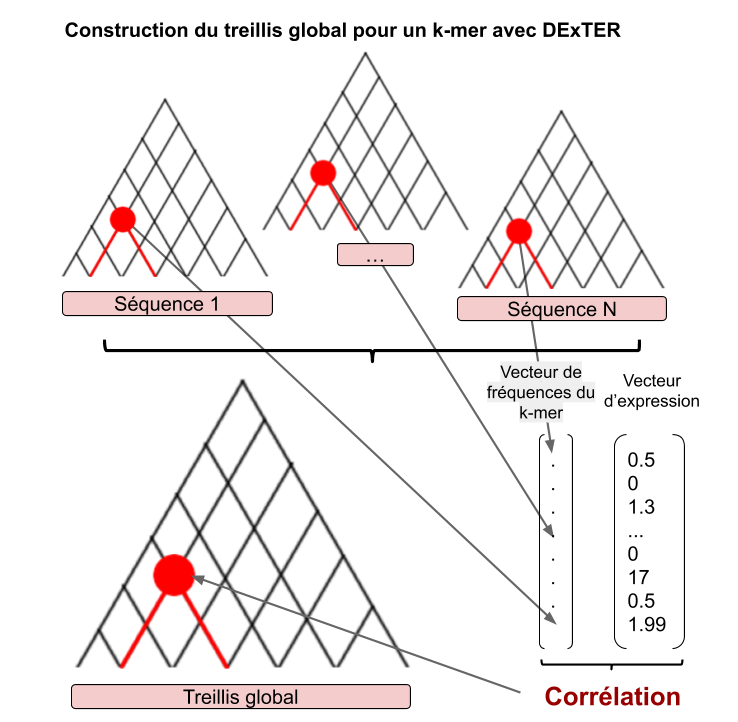
\includegraphics[width=0.7\linewidth]{Images_Dextra/Treillis_global_DExTER.png}
 \caption{Calcul de la corrélation d'un domaine avec un vecteur d'expression $Y$. Le vecteur des taux de k-mer pour toutes les séquences et une région $r$ donnée est obtenu à partir des treillis de chaque séquence individuelles. Ces treillis individuels sont tels que celui présenté en figure \ref{fig/treillis}. Un treillis global est ainsi construit comportant le score de corrélation entre le vecteur de taux du k-mer considéré sur la région $r$ de toutes les séquences, et $Y$ . Il permet de visualiser la corrélation d'un k-mer à la variable réponse sur l'ensemble des séquences à disposition.}
 \label{fig:treillis_global_dexter}
\end{center}
\end{figure}



\begin{figure}[h]
\begin{center}
 	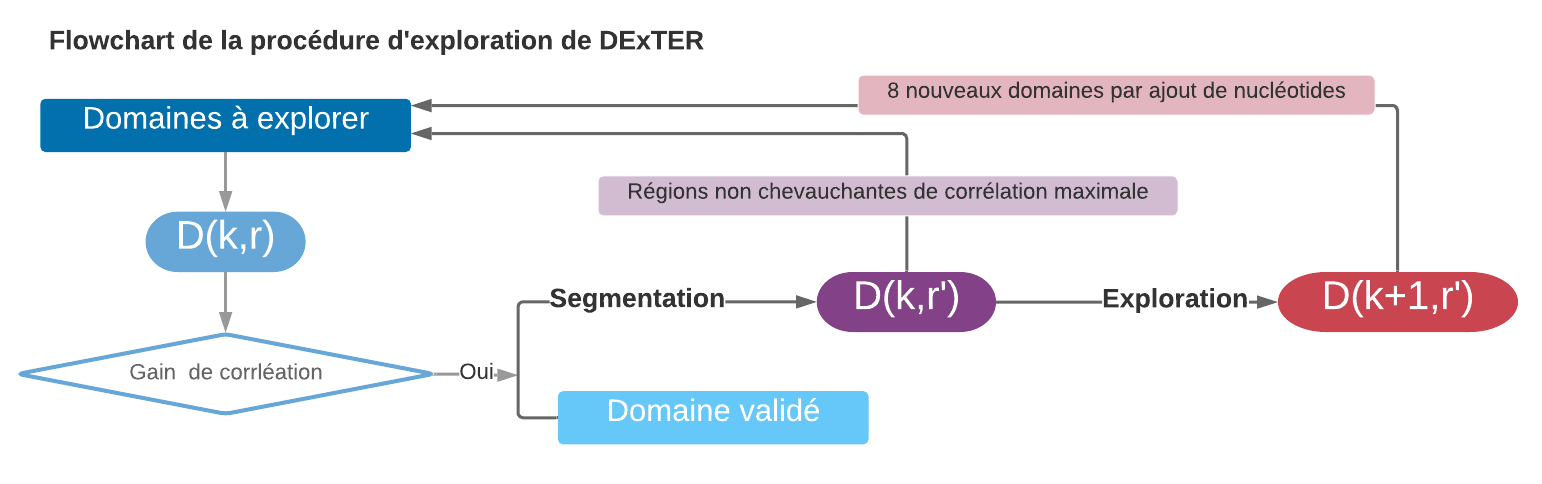
\includegraphics[width = 1\textwidth]{Images_Dextra/DExTER_Flow.png}

 \caption{Schéma représentant le flow d'information au cours de l'exploration des domaines par DExTER. Les domaines sont testés en termes de corrélation à $Y$, et s'ils présentent meilleure corrélation que celle de leurs parents, ils sont étendus ou segmentés pour créer de nouveaux domaines à tester.}
 \label{fig:dexter_flow}
\end{center}
\end{figure}


\subsubsection{DExTRA} \label{section:dextra}



Nous avons souhaité adapter la méthode de DExTER à la problématique de proximité spatiale des régions régulatrices. L'objectif est de pouvoir extraire des variables expliquant au mieux les contacts entre les promoteurs des gènes dans le noyau d'une cellule, plutôt que l'expression des gènes comme le fait la version originale.


Cette adaptation de DExTER, nommée DExTRA (Domain Exploration To explain chromosomic Regions Associations) a donc pour objectif de traiter des paires de promoteurs pour en prédire l'interaction dûe au repliement spatial de la molécule d'ADN. Pour cela, des données contenant un ensemble de paires et les contacts associés sont données à l'algorithme en tant que vecteur à prédire $Y$.

\paragraph{Jeu de données}

Les données utilisées ici sont les données issues de Chia-Pet. Ces données ont été traitées différemment de ce qui a été décrit en partie \ref{section:chia-pet}. Pour s'adapter à la problématique des paires promoteur-promoteur, c'est une matrice de contacts qui a été créée. La liste des promoteurs impliqués dans des interactions chromosomiques a été faite, puis une matrice répertoriant le nombre de contacts entre ces promoteurs deux à deux, également appelés \textit{counts}, a été construite. Cette matrice, extrêmement \textit{sparse}, se remplit essentiellement autour de sa diagonale, mettant en contact des régions déjà proches dans l'ordre chromosomique. Ces contacts plus distants sont également visibles, de manière symétrique autour de cette diagonale. Un ensemble de paires peut donc être constitué, en échantillonnant des couple de promoteurs avec une distribution en \textit{counts} la plus uniforme possible. Nous sélectionnons également à l'aide de cette matrice la même quantité de paires de promoteurs ayant une valeur nulle de \textit{counts}, afin de représenter les paires de \textit{background}. Enfin, ces \textit{counts} sont binarisés, pour associer à une paire la valeur 1 si il existe des interactions spatiales entre les deux promoteurs, et 0 sinon. Au total, 8269 paires constituent ce vecteur. 

\paragraph{Adaptation de l'algorithme DExTER}

Le principe d'exploration des séquences, leur segmentation et la validation des domaines informatifs sont conservés par rapport à DExTER. Dans DExTRA, la différence intervient dans le critère à maximiser pour sélectionner ou non un domaine lors de cette exploration. Alors que DExTER mesure une corrélation entre les fréquences de k-mer d'une liste de séquences et les expressions relatives à chacune de ces séquences lors de la construction d'un treillis global, DExTRA utilise un score différent. Ce score doit renseigner sur le niveau d'information apporté par les fréquences en k-mer des deux promoteurs d'une paire quant à leur mise en contact ou non.

La liste de paires obtenues après le traitement des données de ChIA-Pet est donc fournie à DExTRA. Pour chaque domaine $D_{k,r}$ rencontré lors de l'exploration, on calcule un vecteur valant la valeur absolue de la différence du taux de $k$, k-mer associé au domaine. Cela fournit un vecteur caractérisant les paires de promoteurs, par une grandeur représentant leur similarité en termes de fréquence de $k$ sur la région $r$. Ce vecteur doit ensuite être comparé à la variable réponse, l'interaction ou non des promoteurs de la paire, modélisé par $Y$. $Y$ étant binaire, une mesure de corrélation comme le faisait DExTER n'est pas envisageable. C'est donc une mesure d'AUC sous la courbe ROC qui est utilisée. Cette mesure, usuellement utilisée pour évaluer la qualité des prédictions quantitatives d'un modèle par rapport au vecteur à deux classes attendu, peut également être utilisée ici. Cela revient à estimer la pertinence d'un modèle à une seule variable, ici la différence en valeur absolue des taux de $k$ sur $r$, pour prédire la variable réponse.

Par conséquent, la procédure de construction d'un treillis de score global est modifiée, telle que montrée en figure \ref{fig:treillis_global_dextra}.

\begin{figure}[h]
\begin{center}
 	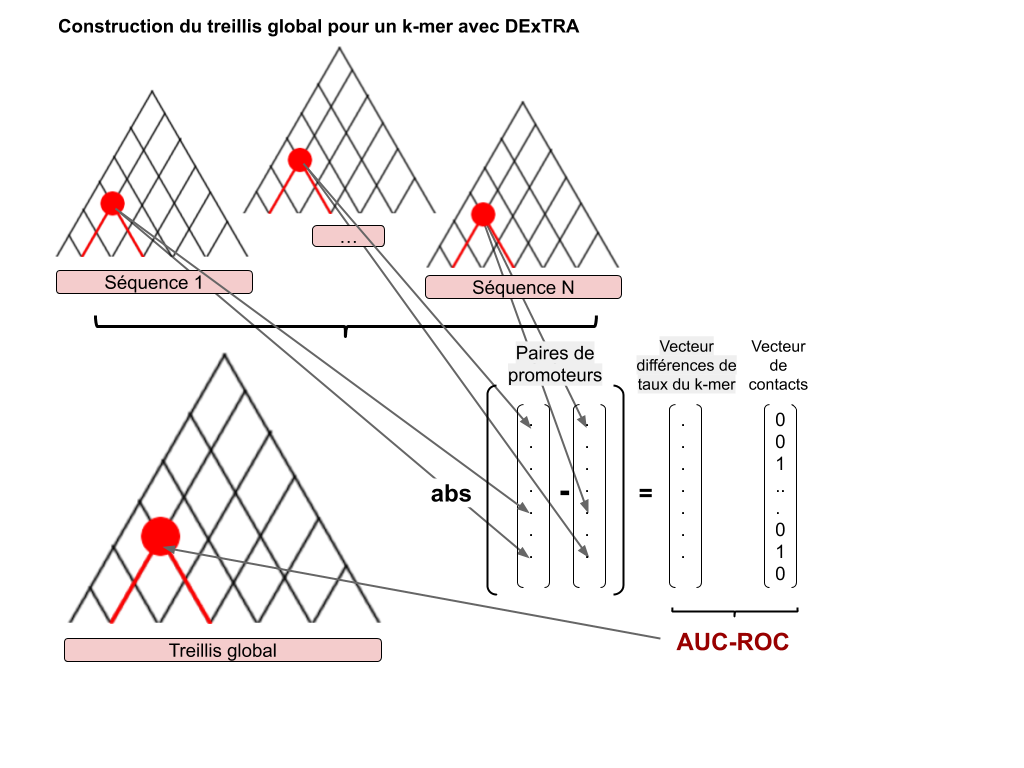
\includegraphics[width=1\linewidth]{Images_Dextra/Treillis_global_DExTRA.png}
 \caption{Calcul de l'AUC d'un domaine avec un vecteur de contacts $Y$. Le vecteur des taux de k-mer pour toutes les séquences et une région $r$ donnée est obtenu à partir des treillis de chaque séquence individuelles. Ces treillis individuels sont tels que celui présenté en figure \ref{fig/treillis}). Un treillis global est ainsi construit comportant le score d'AUC entre le vecteur de différence en valeur absolue des taux du k-mer considéré sur la région $r$ de toutes les séquences, et $Y$. Il permet de visualiser le score prédictif d'un k-mer par rapport à la variable réponse sur l'ensemble des paires positives ou négatives formées.}
 \label{fig:treillis_global_dextra}
\end{center}
\end{figure}

\paragraph{Classification}

A l'issue de la méthdoe DExTRA, nous obtenons un ensemble variables dont les valeurs dans les paires d'entraînement optimisent la prédiction des contacts entre promoteurs. Le finalité de cette procédure d'extraction de \textit{features} est de les combiner dans un modèle, qui sélectionnera les plus importantes, afin de prédire au mieux les interactions chromosomiques. Les modèles décrits en section \ref{section:models} sont alors envisagés dans deux configurations différentes, présentées en figure \ref{fig:dataset_configs} :

\begin{itemize}
    \item 1. Pour chaque paire, la valeur absolue de la différence est donnée pour toutes les variables extraites par DExTRA, afin de prédire le vecteur de \textit{counts} binaire.
    \item 2. Pour chaque paire, la valeur de toutes les variables extraites par DExTRA  est donnée pour le premier promoteur de la paire, ainsi que pour le second, afin de prédire le vecteur de \textit{counts} binaire.
\end{itemize}

\begin{figure}[h]
\begin{center}
 	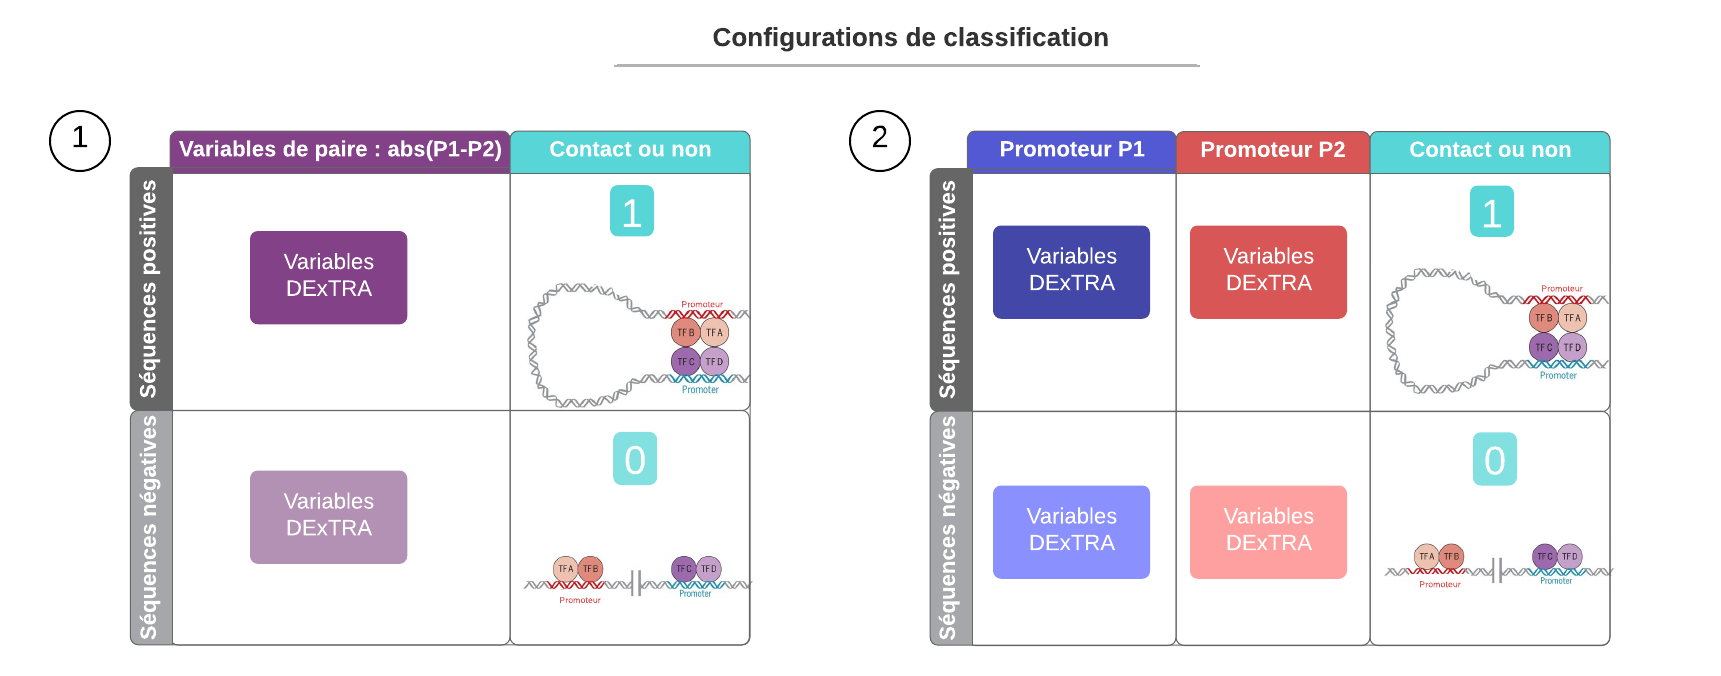
\includegraphics[width=1\linewidth]{Images_Dextra/Dataset_promoters.png}
 \caption{Différents jeux de données utilisés pour entraîner et tester les modèles.}
 \label{fig:dataset_configs}
\end{center}
\end{figure}

Ces deux configurations permettent de tester les manières de présenter les variables aux modèles de classification. Ayant été extraites en utilisant la valeur absolue de la différence des fréquences de k-mer comme critère de sélection, un modèle prenant en compte directement cette opération pour chaque paire sera-t-il intéressant? Le sera-t-il plus qu'on modèle construit sur les valeurs des domaines pour chaque membre des paires séparément? En effet, cette dernière option permet de laisser les modèles les combiner à leur manière.

Les jeux d'entraînement et de tests sont, comme précédemment, construits en utilisant pour l'entraînement des paires ne partageant pas d'élément en commun avec les paires de test.
\section{Résultats}

\subsection{Prédiction des interactions enhancer-promoteur} \label{section:res_EP}

Cette section rend compte des résultats liés au méthodes de la section \ref{section:methdoes_ep}, visant à prédire les interactions de paires enhancers- promoteurs. Ces prédictions sont faites sur les compositions en nucléotides et les motifs PWM sur l'ensemble des séquences, sans segmentation, et sur le jeu de données de la figure \ref{fig/dataset}.



\paragraph{Étude du problème de classification}
Tout d'abord, nous avons considéré deux manières de construire les paires positives et négatives, formant deux problèmes différents, décrits en \ref{section:methdoes_ep}. Pour étudier ces deux cas, 300 modèles de classification ont été entraînes, chacun sur un type cellulaire représenté dans les données FANTOM. Ces modèles sont construits en prenant comme variables les compositions nucléotidiques de l'enhancer et du promoteur.

Le problème consistant à prédire les paires dont l'enhancer est actif contre celles dont l'enhancer est inactif s'est avéré plus évident à prédire en classification. Le second problème, prédisant l'expression simultanée contre seulement l'un des membres exprimés dans la paire, présente des AUC inférieures. Nous constatons que ces résultats sont cohérents suivant les modèles utilisés : qu'il s'agisse des la régression logistique pénalisée (Lasso), des \textit{Random Forests}, ou du \textit{Stochastic Gradient Boosting}, les distributions d'AUC sont comparables pour un problème donné.

\begin{figure}[h]
\begin{center}
 	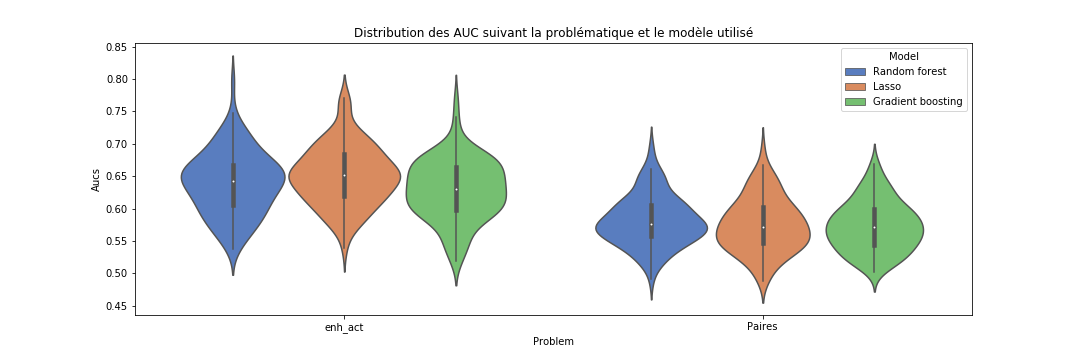
\includegraphics[width=1\linewidth]{Images_FANTOM/AUC_problems_models.png}
 \caption{Valeurs d'AUC pour les différents problèmes : prédiction de l'activité des enhancers (gauche), ou prédiction des paires enhancers-promoteurs (droite).} \label{fig/treillis_at}
\end{center}
\end{figure}

Cette différence de performances entre les problèmes s'explique par le fait qu'il est plus facile de prédire l'activité d'un enhancer à partir de sa séquence, que l'appariement de deux régions régulatrices de nature différentes. Les AUC de ce dernier problème, légèrement supérieures à 0.5, suggèrent que les prédictions de tels contacts ne peuvent pas être faites sur la bases des compositions nucléotidiques uniquement.
Nous étudions par la suite ce problème dans un type cellulaire précis.

\paragraph{Étude des variables} 


La construction du jeu d'apprentissage précédemment décrit permet l'étude des importances relatives des variables de l'enhancer et du promoteur, des variables de fréquences nucléotidiques aux PWM, de l'ajout de variables de paires, en comparant les performance de prédiction des contacts. 
La construction d'un modèle avec la composition en nucléotides a donc été comparée avec un modèle utilisant la composition en nucléotides et les scores PWM, à la fois pour l'enhancer et le promoteur. Les figures \ref{fig:rocs_fantom_ep_nucl} et \ref{fig:rocs_fantom_ep_nucl_pwm} montrent les résultats de telles classifications en prenant en compte ou non les PWM.

\begin{figure}[!htb]
    \centering
    \begin{minipage}[t]{.5\textwidth}
        \centering
        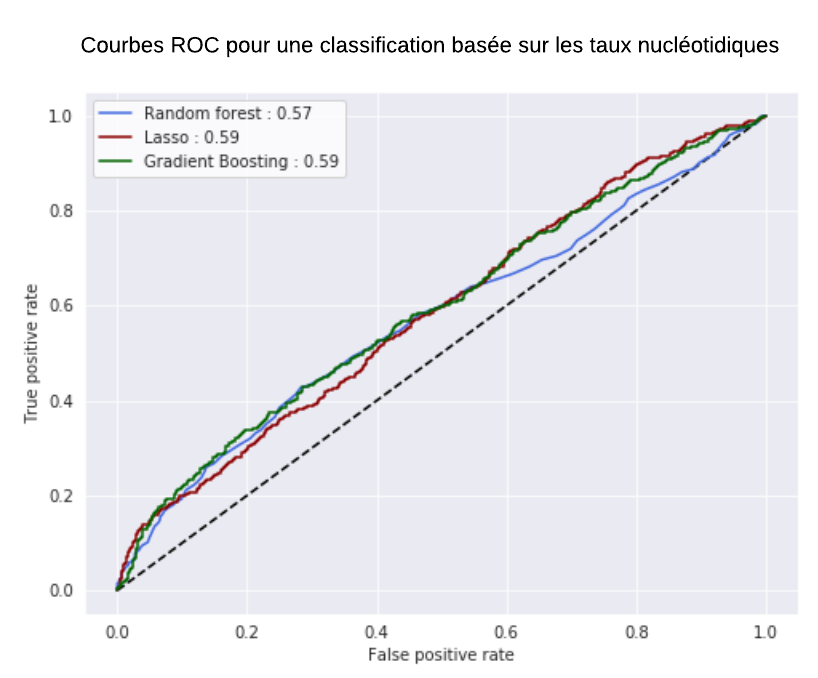
\includegraphics[width=1\linewidth]{Images_FANTOM/rocs_fantom_ep_nucl.png}
        \caption{Courbes ROC et AUC pour un modèle entraîné sur les variables de taux de nucléotides des enhancers et des promoteurs}
        \label{fig:rocs_fantom_ep_nucl}
    \end{minipage}%
    \begin{minipage}[t]{.5\textwidth}
        \centering
        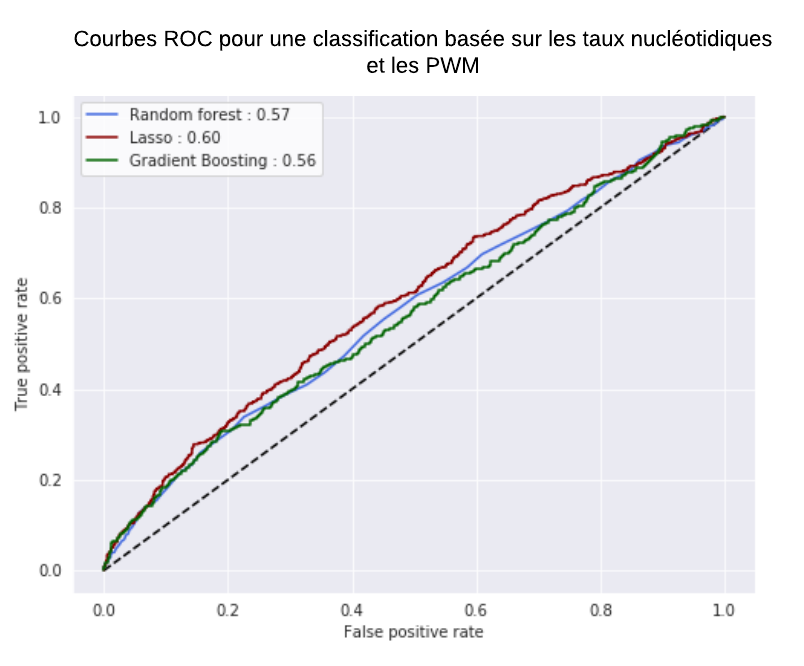
\includegraphics[width=1\linewidth]{Images_FANTOM/rocs_fantom_ep_nucl_pwm.png}
        \caption{Courbes ROC et AUC pour un modèle entraîné sur les variables de taux de nucléotides et les scores PWM des enhancers et des promoteurs}
        \label{fig:rocs_fantom_ep_nucl_pwm}
    \end{minipage}
\end{figure}

Les AUC sont également faibles, légèrement supérieures à un \textit{classifier} aléatoire.
L'ajout des scores PWM ne semble pas informatif par rapport à l'appariement de ces séquences régulatrices, pouvant même conduire à une perte de performances causée par un grand nombre de variables non utiles.

Nous avons également construit des modèles utilisant uniquement les enhancers ou les promoteurs, pour déterminer si les variables de l'un ou de l'autre peuvent être prépondérantes dans l'information. La table \ref{tab_aucs_fantom_ep} référence les valeurs d'AUC et montre que c'est majoritairement les variables de l'enhancer qui déterminent le faible signal prédictif.

\begin{table}[ht]
 \begin{center}
   \begin{tabular}{l | c c c}
   \hline
           Variables nucléotidiques pour :     & Lasso & Random Forest & Gradient Boosting  \\
   \hline
    Enhancer et promoteur & 0.59        & 0.57   &    0.59\\
    Enhancer        & 0.59   &    0.56  & 0.56\\
    Promoteur        & 0.50   &    0.50 & 0.52\\
   \hline
\end{tabular}
\caption{Valeurs d'AUC pour les différents \textit{classifiers} et différents membres des paires injectés dans le modèle.}
\label{tab_aucs_fantom_ep}
 \end{center}
\end{table}

Nous avons ensuite appliqué ce modèle aux données de ChIA-PET. Dans ce cas, les paires négatives sont les paires positives randomisées. Nous avons donc construit des modèles avec les variables simples (colonnes rouge  et bleue de la figure \ref{fig/dataset}), puis ces mêmes modèles avec, en plus, des variables de paires (toutes les colonnes de la figure \ref{fig/dataset}). Les résultats sur le modèle de base, avec les variables de nucléotides pour l'enhancer et le promoteur confirment ceux obtenus avec les paires FANTOM, comme le montre la figure \ref{fig:rocs_chia_simple}, avec des AUCs entre 0.53 et 0.54. L'ajout des variables de paire au jeu de données, montré en annexe 3, figure \ref{fig:rocs_chia_int} n'a pas permis d'amélioration des prédictions, avec des AUCs également comprises entre 0.53 et 0.54. 

Les autres fonctions utilisées pour créer des variables d'interactions se sont montrées tout aussi peu informatives sur cette problématique. Sur cette partie, apparaît une réelle concordance des résultats entre les données FANTOM et les données de ChIA-PET : qu'il s'agisse d'un appariement inféré par corrélations, ou des contacts exhibés par expériences biologiques, il semblerait que les variables de séquenece étudiées ne permettent pas de prédire le repliement de la chromatine.

\paragraph{Validation sur un jeu de données artificiel}
 Afin de s'assurer de la validité des modèles développés, nous avons souhaité les tester sur des jeux de données fictif. Les taux du score PWM d'un certain facteur de transcription, ATF1, ont été modifiés de manière à ce que les scores de l'enhancer et du promoteur soient proches dans les paires positives, et inchangés dans les paires négatives. La modélisation est la suivante : pour toutes les paires labellisées en contact, la valeur de score du promoteur a une probabilité $p$ de suivre une loi normale centrée en la valeur de l'enhancer, et d'écart type 0.1. Les modèles de classification sont alors construits, incluent les taux de PWM et dinucléotides pour l'enhancer et le promoteur, ainsi que le \textit{logratio} de ces deux valeurs. Avec une probabilité $p = 0.9$, cette composition similaire est bien visible est captée par les modèles, comme le montre la figure \ref{fig:fictif} en annexe 4, graphe de sélection des variables lors de la régression logistique pénalisée.


Les autres modèles classent également cette variable de paire relative à ATF1 comme la plus importante. Les AUCs de classification sont alors extrêmement hautes, excédant 90\%, car l'information insufflée au dataset pourrait être plus subtile (en faisant notamment varier $p$). Nous en concluons que lorsque les données comportement de l'information discriminant les paires en contact des autres, les \textit{classifiers} sont capables de la détecter.

\subsection{Prédiction des interactions promoteur-promoteur par extraction de \textit{features}}\label{section:res_dextra}

Dans cette section, sont présentés les résultats obtenus avec la méthode DExTRA, présentée en section \ref{section:dextra}. A la suite d'une exploration par fractionnement des séquences, des domaines associant un k-mer à une région de la séquence sont retournés, et sensés expliquer au mieux individuellement les appariements promoteur-promoteur observés dans les données de ChIA-PET. Ces variables sont ensuite injectées dans un modèle global pour prédire les contacts en combinant toutes ces variables. Nous avons dans un premier temps pensé à des régions chromosomiques de taille similaire à celles de la partie précédante : $\pm 500 bp$ autour du centre du promoteur. Nous avons cependant souhaité élargir ces régions $\pm 10000 bp$, afin d'être sûr de ne manquer aucune information, laissant à DExTRA la liberté de choisir des domaines plus restreints au besoin.
Les résultats sont relativement surprenants. En effet, lors de l'exploration des domaines, DExTRA génère des treillis globaux avec l'AUC des k-mers par rapport à la réponse sur l'ensemble des séquences, comme celui montré en figure\ref{fig/treillis_at}. Plus les AUC sont hautes sur une région, plus cette région explique les contacts chromatiniens. Ici, plutôt que de montrer des AUC fortes sur la région promotrice, que l'on supposait jusqu'ici informative sur les contacts, c'est son voisinage qui semble explicatif. L'AUC maximale est obtenue au sommet du treillis, car le sommet combine l'information du voisinage amont et aval du promoteur. Un zone "morte", avec peu d'informations apportée sur la réponse à prédire est située au centre de la séquence, là où se situe le promoteur.

\begin{figure}[h]
\begin{center}
 	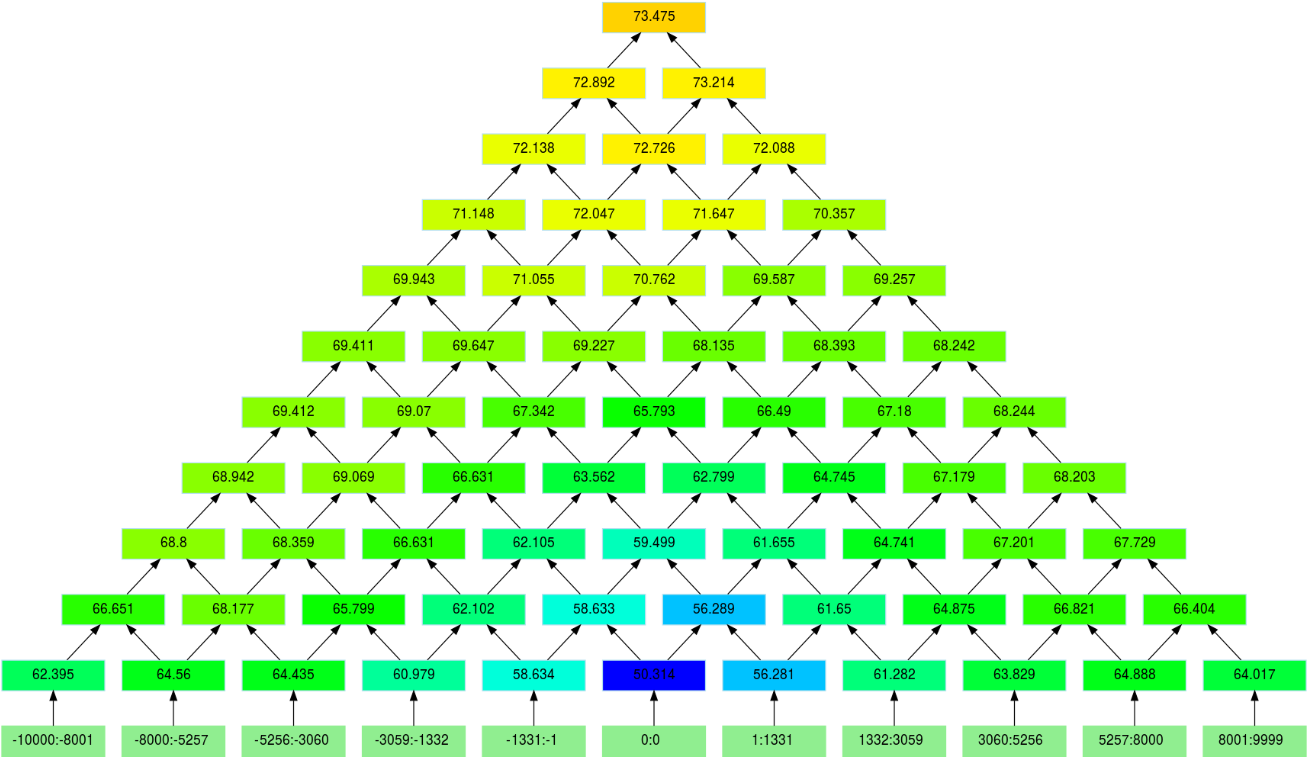
\includegraphics[width=1\linewidth]{Images_Dextra/AT_low.png}
 \caption{Treillis global d'AUC pour le dinucléotide AT obtenu lors de l'exploration de DExTRA. Les couleurs les plus chaudes indiquent un valeur d'AUC plus forte pour le k-mer sur le noeud considéré.} \label{fig/treillis_at}
\end{center}
\end{figure}

Ce pattern montrant un centre peu informatif contrairement à son entourage ne se retrouve pas avec tous les k-mers, mais avec ceux qui traduisent le taux de GC (proportion de nucléotides, à ne pas confondre avec des taux de dinucléotides, G ou C dans les séquences, valant 1 moins le taux de AC). On parle de \textit{GC content}. Les dinucléotides impliqués dans le \textit{GC content} et exhibant ce \textit{pattern} sont en l'occurence AT, TA, GC, CG, TT, AA, CC et GG. Les k-mer mélangeant purines (A et T) ou pyrimidines (C et G) sont à l'origine de treillis uniformes.
Nous pouvons donc en conclure que c'est probablement l'information des TAD qui est captée par l'extraction de \textit{features} : ces domaines regroupant les gènes actifs simultanément sont connus pour avoir des compositions en nucléotides proches. On parle ici d'isochores, de longues régions de l'ADN, d'au moins 300 kbp, uniformes en termes de \textit{GC content}.

Certains k-mers de taille plus élevée sont également sélectionnés, toujours sur l'ensemble de la séquence.

L'ensemble des domaines sélectionnés par DExTRA sont visibles dans le graphe d'exploration de la figure  \ref{fig:explo} de l'annexe 5.

Les domaines sélectionnés sont ensuite utilisés comme variables explicatrices dans les modèles utilisés jusqu'ici. Les paires d'apprentissage sont celles utilisées lors de l'exploration de DExTRA pour mesurer les AUC, et les paires de test sont celles n'ayant aucun promoteur en commun avec les paires de \textit{training}. Les deux configurations mentionnées en \ref{fig:dataset_configs} de la section \ref{section:dextra} (variables simples et variables de paire uniquement) sont testées, et fournissent les résultats de la table \ref{tab_aucs_dexter}. Les courbes ROC de chacune des configurations se retrouvent en figure \ref{fig:aucs_dextra_configs}.

\begin{table}[ht]
 \begin{center}
   \begin{tabular}{l | c c c c}
   \hline
                & Lasso & Random Forest & Gradient Boosting & Perceptron multicouche \\
   \hline
    (1) & 0.629        & 0.799   &    0.774 & 0.760\\
    (2) & 0.737        & 0.772   &    0.744 & 0.743\\
   \hline
   \end{tabular}
   
\caption{Valeurs d'AUC pour les différents \textit{classifiers} et les configurations de variables testées.\\
(1) : Taux pour chaque promoteur de la paire\\(2) : Différence en valeur absolue des deux taux}  \label{tab_aucs_dexter}
 \end{center}
\end{table}

Les variables sélectionnées par chacun de ces modèles concordent avec les variables montrant la plus forte AUC dans le graphe d'exploration, c'est à dire les k-mer traduisant le \textit{GC content}. La figure \ref{fig:imp_rf} de l'annexe 6 montre l'ordre d'importance des variables pour les \textit{Random Forests} pour chacune des configurations.

Ces deux différentes configurations sont très intéressantes quant au comportement et à la nature des modèles en jeu. En effet, lorsque l'on donne à la régression logistique les taux de k-mer pour chacun des promoteurs de la paire sans en faire la différence en valeur absolue, les performances sont clairement inférieures à celles des autres modèles, dits non linéaires. L'AUC est de 0.631 pour la regression, et entre 0.76 et 0.799 pour les autres \textit{classifiers}. Lorsque la variable de différence en valeur absolue des taux de k-mers est directement fournie comme dans la seconde configuration, la régression fait tout aussi bien que les autres modèles, montrant ainsi qu'elle ne peut pas traduire combinaison de variables non linéaire.

Un autre résultat est la capacité des \textit{Random Forests} à combiner les variables de taux de k-mers pour chaque membre de la paire, dans la configuration 1, de manière plus informative que celle donnée par la seconde. L'AUC avec les variables pour chaque promoteur est en effet de 0.799 dans la configuration 1, contre 0.774 dans la seconde. On peut en déduire qu'il existe une fonction autre que la valeur absolue de la différence des varuibles, identifiée par les \textit{Random Forests}, permettant une meilleure classification des paires en contact.

\section{Perspectives et discussions}

Au cours de ce stage, il a été montré que la prédiction de la mise en contact de régions génomiques régulant la transcription est un mécanisme encore complexe à prédire. Afin de construire une approche correcte, il est nécessaire de s'inspirer de la littérature, tout en prenant conscience des erreurs de design expérimental que l'on peut y trouver, et de les inclure à une nouvelle approche.


En considérant la région stricte des promoteurs et des enhancers comme en section \ref{section:res_EP}, les résultats tendent à prouver que des variables de séquence uniquement ne permettraient pas d'expliquer le repliement chromatinien. Cela vaut pour la méthodologie utilisée, mais n'exclue pas un effet de la séquence identifiable grâce à d'autres expériences ou protocoles de recherche. 


Peu de résultats positifs sont obtenus en se basant sur les séquences des enhancers et des promoteurs, mais des constats émergent lorsque nous élargissons la fenêtre d'étude au voisinage chromosomique de ces régions, et que nous prédisons des contacts entre promoteurs comme présenté en section \ref{section:res_dextra}. Des régions sélectionnées à posteriori grâce à une extraction de \textit{features} indiquent finalement que la composition nucléotidique du voisinage des promoteurs a un effet sur leurs interactions plus longues distances. Il pourrait donc être envisagé d'appliquer ce principe de voisinage informatif à la problématique de la première partie, impliquant également les contacts avec les enhancers.

Les difficultés de prédiction de ces interactions peuvent résider dans plusieurs réalités biologiques. La précision et la validité des expériences de ChIA-PET ne sont pas parfaitement établies, et certaines expériences indiquent qu'il y aurait un nombre important de faux positifs dans les contacts détectés. 
 Il a été montré que dans certains cas, chez la drosophile, l'expression des gènes ne dépend pas de la conformation tri-dimensionnelle de l'ADN \cite{ghavi-helm_highly_2019}. De même, des chercheurs ont observé que chez l'homme, certains enhancers n'ont pas besoin de venir en contact avec un promoteur pour réguler le gène associé, c'est le cas du gène SOX2 par exemple \cite{alexander_live-cell_2019}.

Il reste beaucoup de pistes d'améliorations possibles pour se projet, notamment quant à la méthode DExTRA. Une autre méthode de construction de treillis serait envisageable. En effet, la structure actuelle se base sur les taux de k-mers entre deux points A et B d'une séquence, mais un domaine associé aux bornes A et B pourrait également représenter toute la séquence excluant le segment AB. Ainsi, nous pourrions utiliser des critère d'AUC sur l'amont et l'aval d'une région simultanément. Cela présenterait l'avantage d'obtenir des AUC encore plus hautes, s'affranchissant des zones centrales peu informatives observées.

Nous pourrions également distinguer les contacts intra-chromosomiques des contacts inter-chromosomiques pour voir si leurs prédictions se font aussi bien les unes que les autres, ou si les patterns qui les dirigent sont différents.

Les modèles construits pourraient probablement largement bénéficier de l'ajout de variables épigénétiques relatives à la conformation de l'ADN, sa forme, sa méthylation. Cependant, cela sort du cadre de l'hypothèse de recherche que nous cherchons à vérifier. D'une manière générale, et comme cela apparaît très majoritairement dans la littérature, la séquence génétique et son environnement ne sont pas indépendantes. La compréhension actuelle de ces phénomènes reste floue, et suggère une action réciproque de la séquence et de son environnement structurel. De la même manière, l'expression des gènes semble influencée par la séquence, et l'influencer en retour.


Différentes propriétés des modèles de \textit{machine learning} utilisés ont pu être mises en lumière, notamment au niveau de leur capacité à détecter les interactions de variables les plus adéquates. Ici, les \textit{Random Forests} se sont montrés particulièrement adaptés. L'utilisation du \textit{deep learning} ne s'est pas faite à son plein potentiel. En effet, un réseau de neurones est capable d'extraire lui même des \textit{features} importantes notamment grâce à des couches de convolution directement sur les séquences, mais celles si sont peu intelligibles. Il ne s'agit ici pas de la volonté du projet, dont l'objectif est tout d'abord de sélectionner des variables importantes et faisait du sens en terme de biologie, puis de les injecter dans des modèles prédictifs.


Le travail effectué est un travail exploratoire, donnant naissance à de nombreuses nouvelles réflexions, tant au niveau des méthodes d'extraction de \textit{features}, que sur les techniques de classification. L'apprentissage statistique, de part sa capacité à identifier des \textit{patterns} parmi d'incroyables quantités de données, permet indéniablement d'éclairer les mécanismes moléculaires permettant notre développement, et notre adaptation au monde.


%%%%%%%%%%%% References et annexes

\clearpage\thispagestyle{empty}\addtocounter{page}{-1} 

\bibliographystyle{splncs03} 
\bibliography{biblio.bib}
 \newpage
 \appendix
\section*{Annexes}

\subsection*{1. Valeurs de scores pour de la méthode TargetFinder après correction du biais}


\begin{figure}[h]
\begin{center}
 	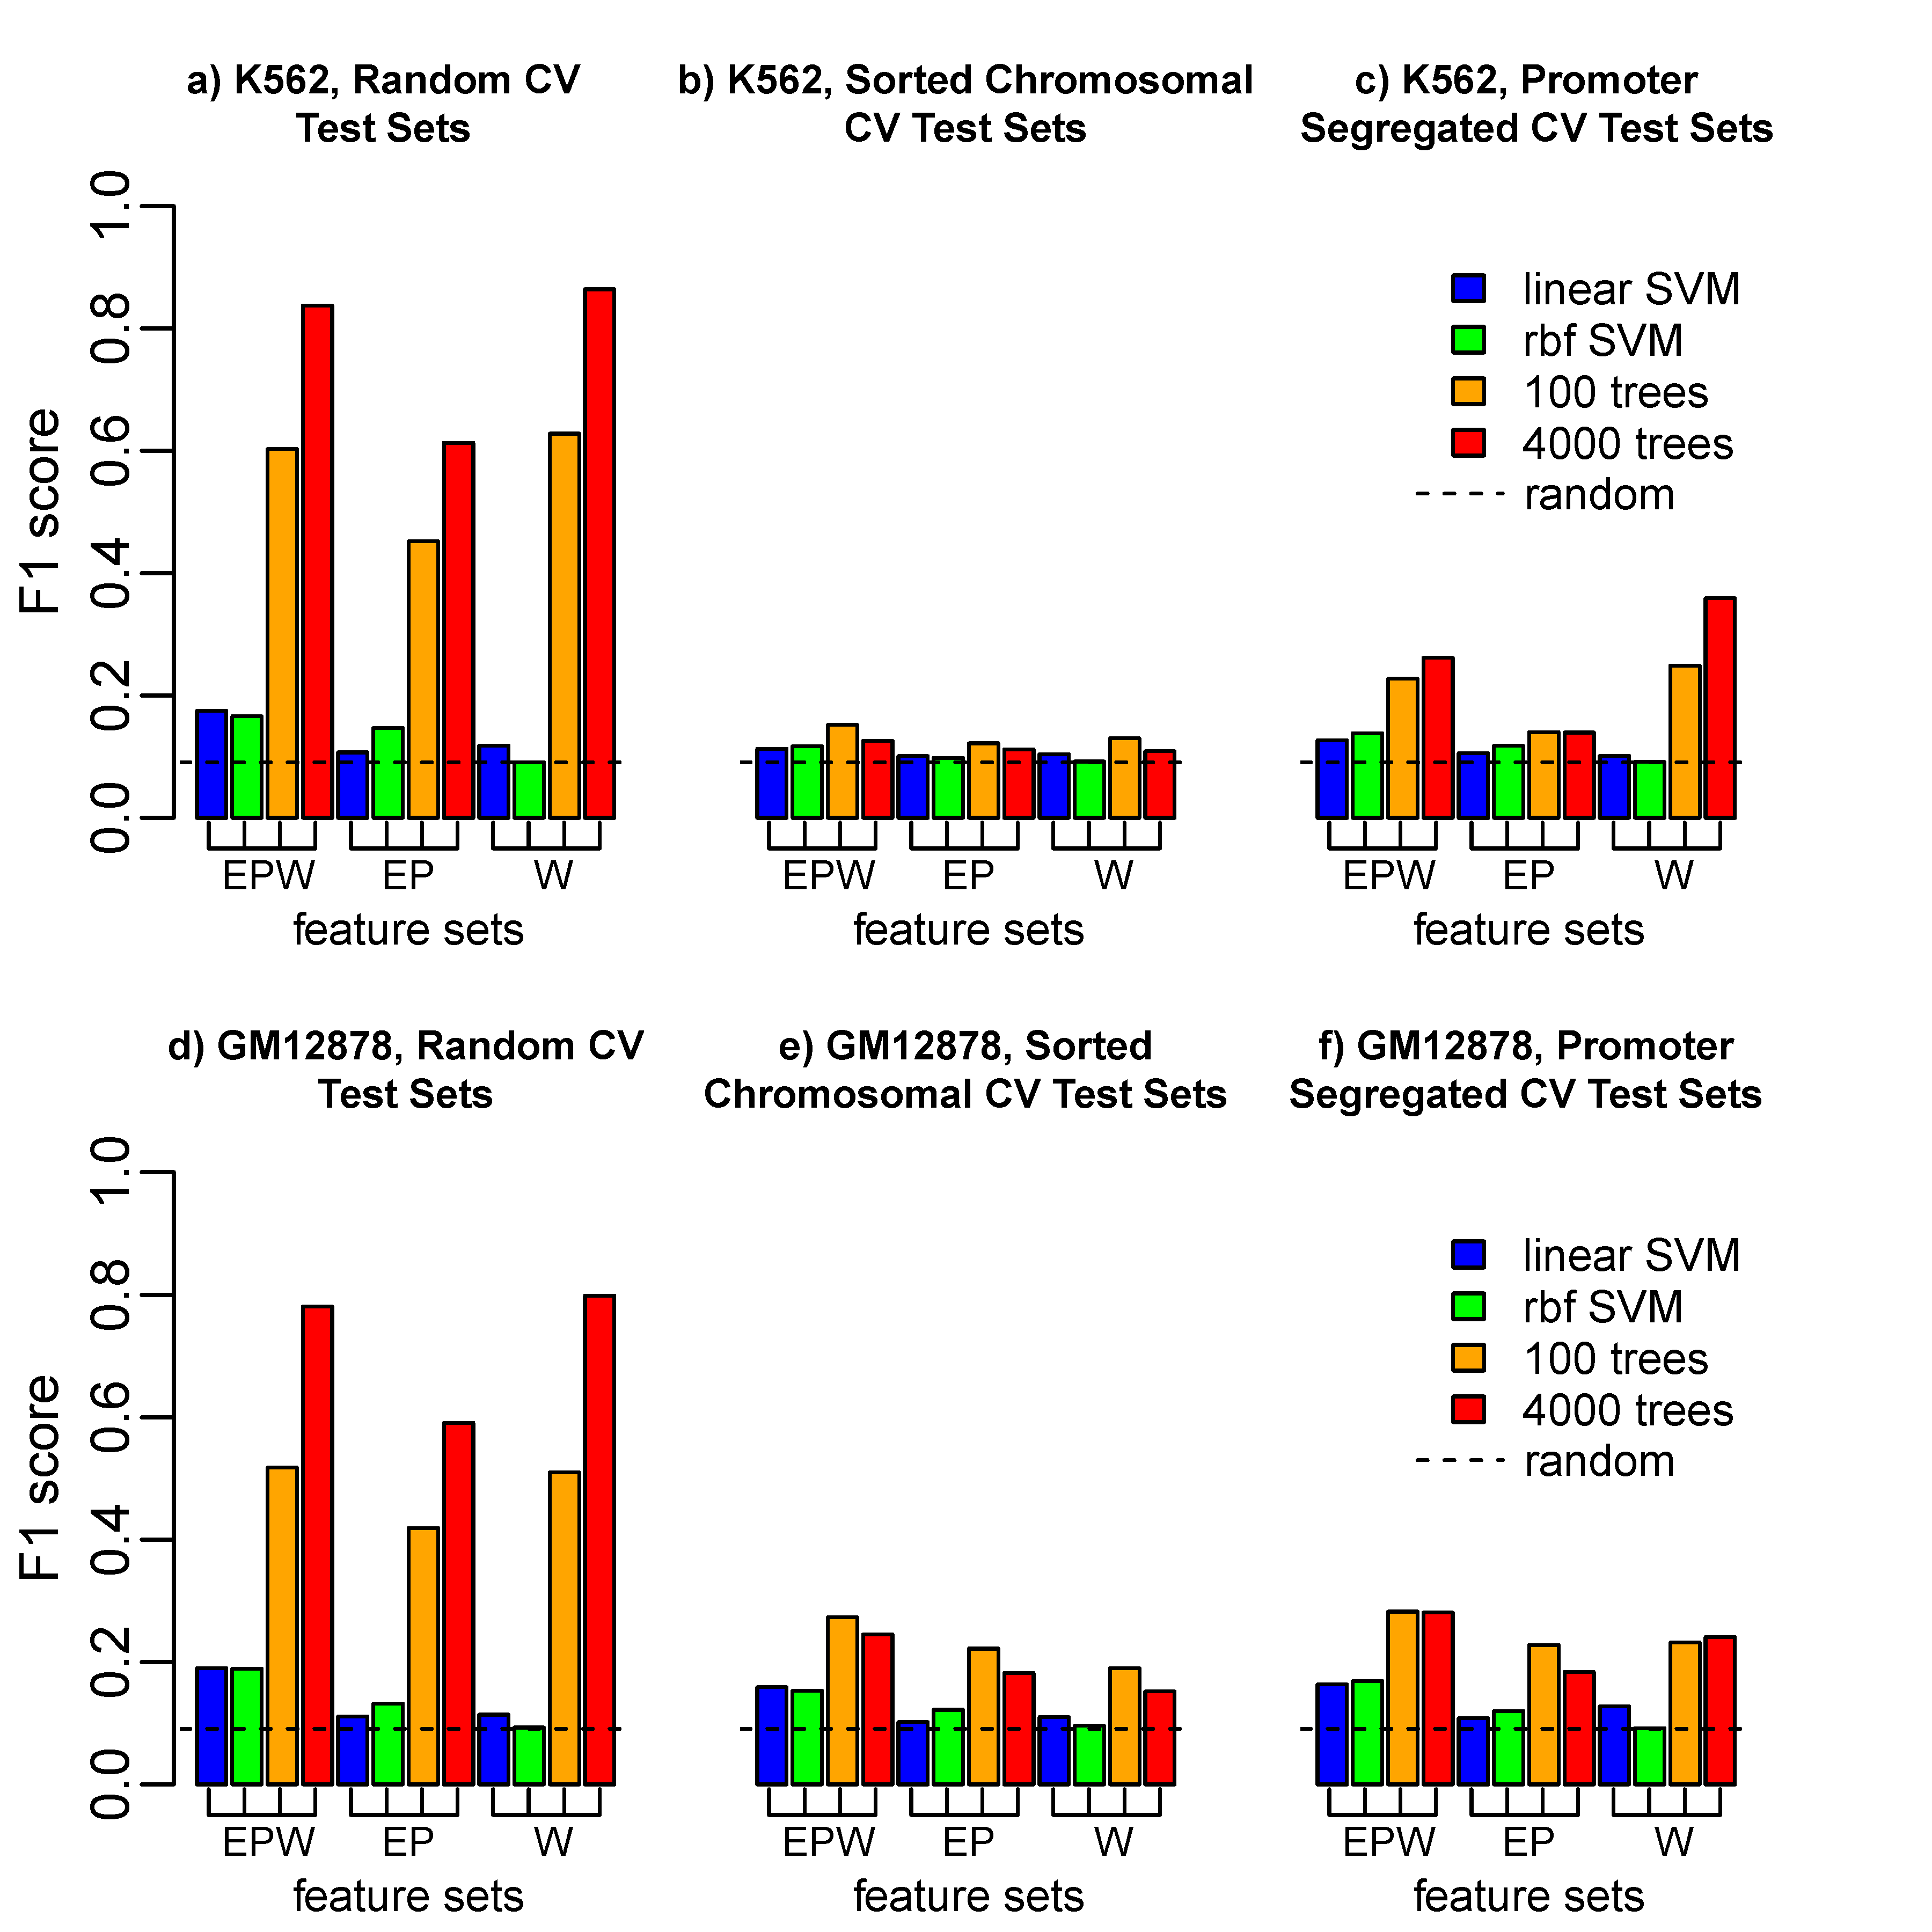
\includegraphics[width=1\linewidth]{Images/xi.PNG}
 \caption{Différence entre les résultats publiés dans TargetFinder à gauche, et la méthode sur un jeu de données de Test issu d'un tri par ordre chromosomique au centre. Nous constatons que les prédictions correctement évaluées ne valent pas plus que le hasard.} \label{fig/correction_biais}
\end{center}
\end{figure}

\newpage
\subsection*{2. Calcul des variables de fréquences nucléotidiques}

La molécule d'ADN est une molécule double brin. La séquence d'un brin est dite  complémentaire de l'autre brin : on passe de l'une à l'autre en remplaçant tous les A par des T, les T par des A, les C par des G, les G par des C. Le brin complémentaire est lu dans le sens inverse du brin direct.
        
Les 16 dinucléotides qu'il est possible de former avec 4 bases n'apparaissent pas tous directement dans les variables utilisées pour caractériser nos séquences, qui sont au nombre de 10. En effet, comme nous considérons une séquence en double brin, compter la fréquence d'un dinucléotide sur les deux brins revient à compter la fréquence de ce dinuclétodide ainsi que celle de son reverse-complément sur un seul brin. Par exemple le taux de AA correspond à la fréquence des AA sur un brin, à laquelle on ajoute la fréquence des TT sur ce même brin. Ainsi, il n'est pas utile de considérer à la fois le taux de AA et de TT dans le modèle, ces informations étant contenues dans une seule de ces deux variables. Un cas particulier est à prendre en compte avec les k-mer pairs. En effet, dans le cas où un k-mer est également son \textit{reverse-complement} (e.g AT, CG, ATAT, CCGG...), sa fréquence en double brin est directement donnée par sa fréquence en simple brin.

Les variables utilisées pour construire les modèles sont donc 6 dinucléotides comprenant aussi leur reverse-complément dans le cas normal, et les 4 dinucléotides considérés comme des cas particuliers (AT, TA, CG et GC). A cela nous rajoutons le AT content et le GC content, qui sont eux des taux de nucléotides, et non des dinucléotides, pour arriver à un total de 12 variables nucléotidiques.

\newpage

\subsection*{3. Prédiction des contacts de ChIA-PET enhancers-promoteurs dans K562 : ajout des variables de paire}

\begin{figure}[!htb]
    \centering
    \begin{minipage}[t]{.5\textwidth}
        \centering
        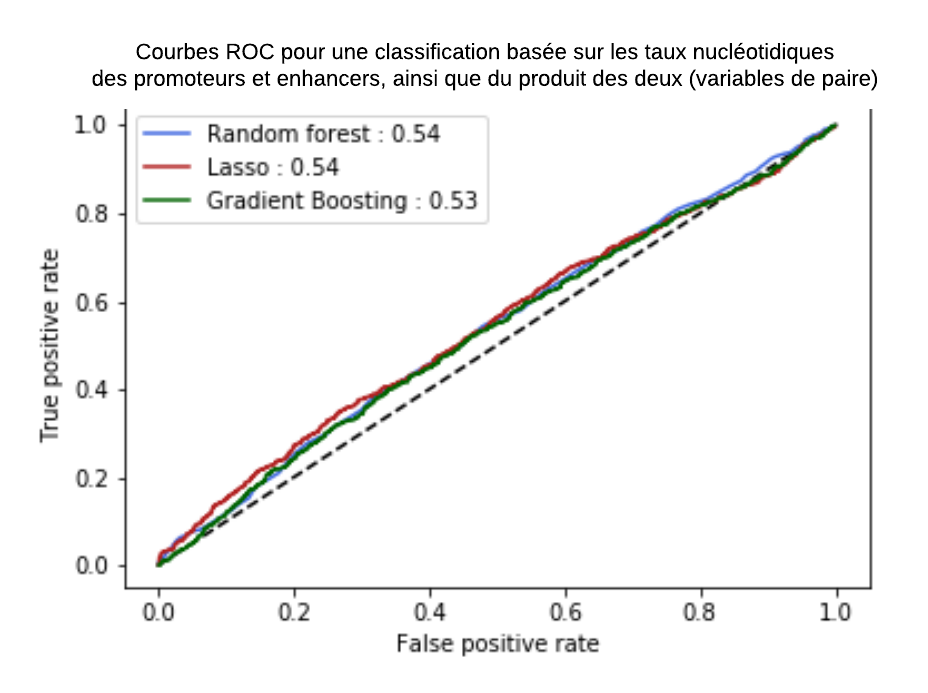
\includegraphics[width=1\linewidth]{Images_FANTOM/rocs_chia_simple.png}
        \caption{Courbes ROC et AUCs pour des modèles entraînés sur les variables de taux de nucléotides des enhancers et des promoteurs sur les données de ChIA-PET}
        \label{fig:rocs_chia_simple}
    \end{minipage}%
    \begin{minipage}[t]{.5\textwidth}
        \centering
        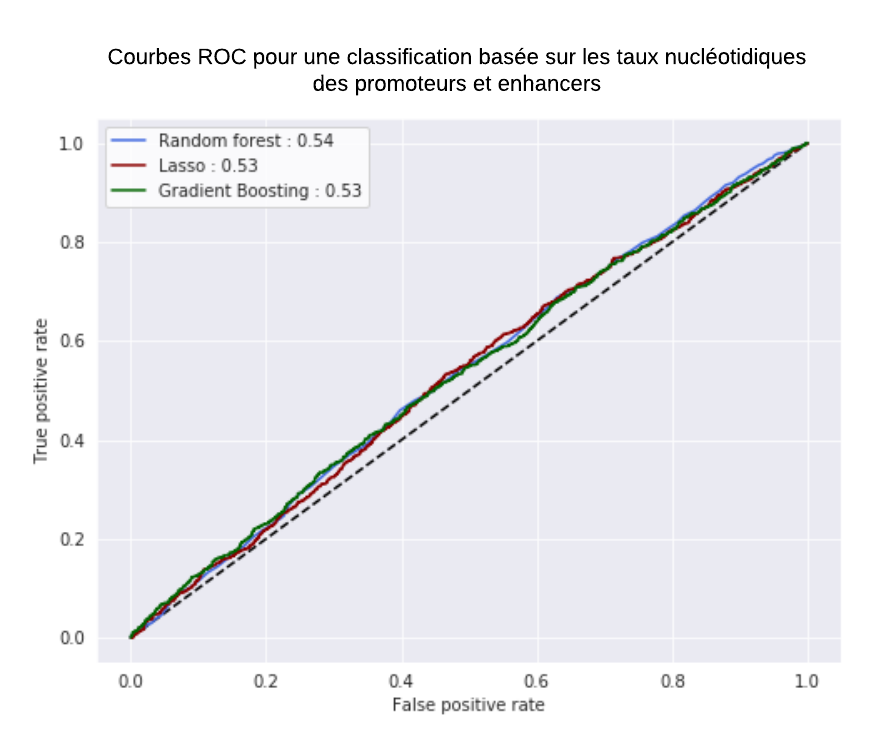
\includegraphics[width=0.9\linewidth]{Images_FANTOM/rocs_chia_inter.png}
        \caption{Courbes ROC et AUCs pour des modèles entraînés sur les variables de taux de nucléotides des enhancers et des promoteurs, ainsi que sur les variables d'interactions : le produit du taux de chaque membre de la paire, sur les données de ChIA-PET.}
        \label{fig:rocs_chia_int}
    \end{minipage}
\end{figure}

\clearpage
\subsection*{4. Sélection de variable sur jeu de données fictif}


\begin{figure}[h]
\begin{center}
 	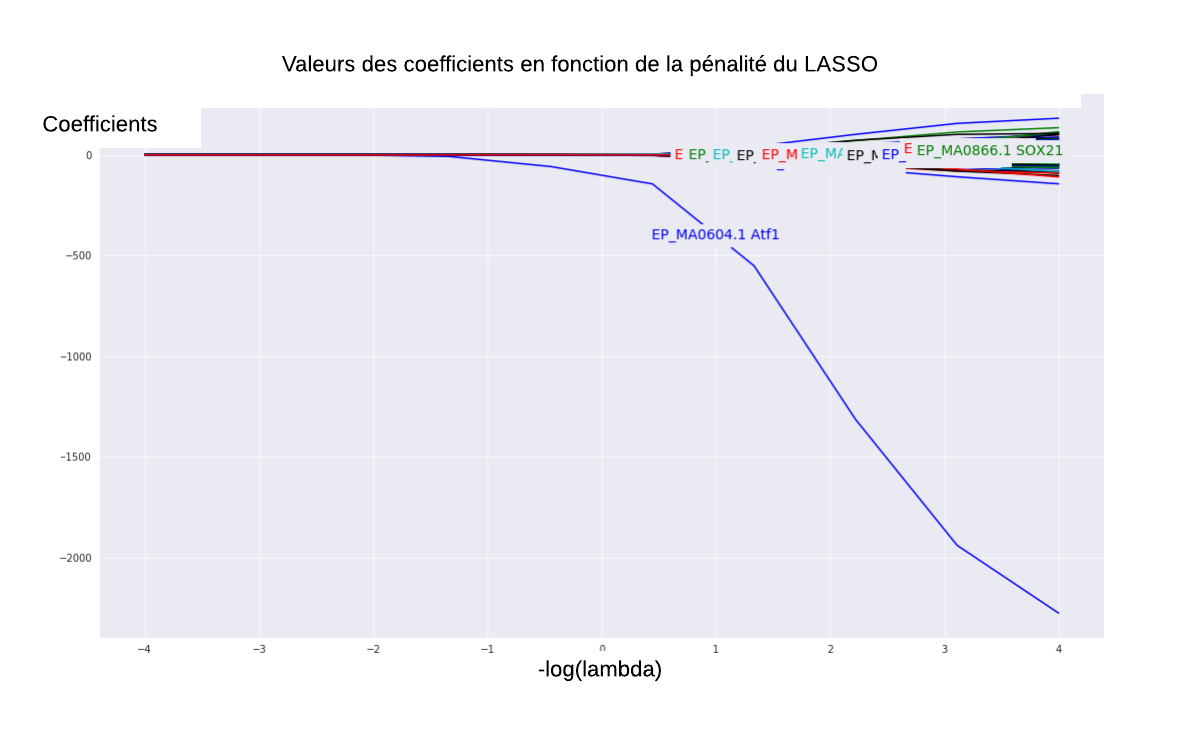
\includegraphics[width=1\linewidth]{Images_FANTOM/Lasso_path_fictive.png}
 \caption{Graphe de sélection de variables lors de la régularisation : lorsque la pénalité est diminuée, la valeur du coefficient relatif à ATF1 est bien celle qui prend en premier une valeur non nulle.} \label{fig:fictif}
\end{center}
\end{figure}

\newpage

\subsection*{5. Graphe d'exploration DExTRA}

\begin{figure}[h]
\begin{center}
 	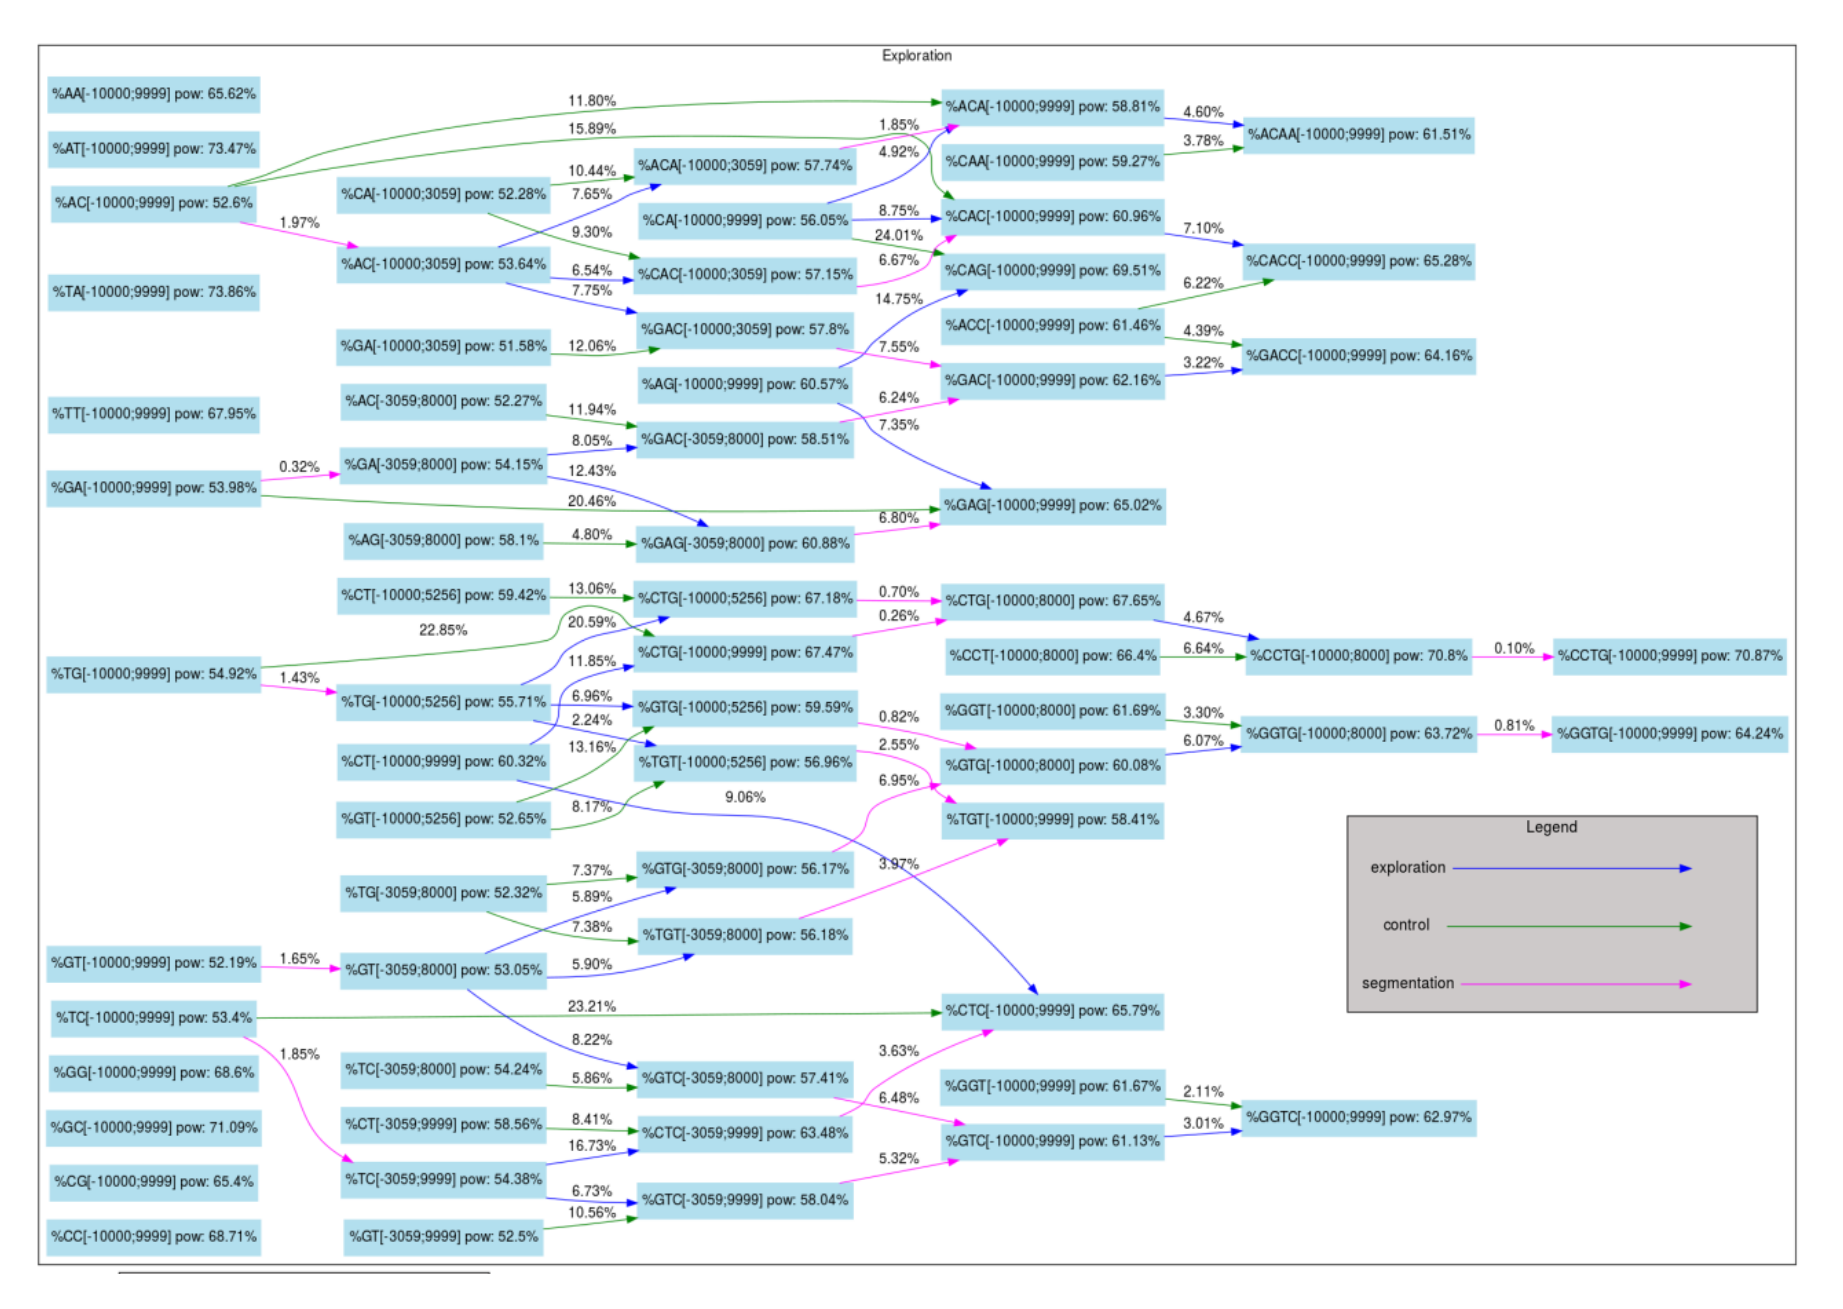
\includegraphics[width=1\linewidth]{Images_Dextra/exploration_graph.png}
 \caption{Graphe d'exploration issu de la procédure DExTRA. Chaque noeud représente un domaine exploré par ajout de nucléotide (flèches bleues) ou refractionné, segmenté (flèches roses). Les flèches vertes représentent les conditions de contrôle mentionnées dans le pseudo-code, au moment de décider de la validation d'un domaine. } \label{fig:explo}
\end{center}
\end{figure}




\subsection*{6. Importance des variables dans les Random Forests pour les deux configurations de variables issues de l'extraction de \textit{features}, et les courbes ROC correspondantes pour tous les modèles}



\begin{figure}[h]
\begin{center}
  \subfigure[1]{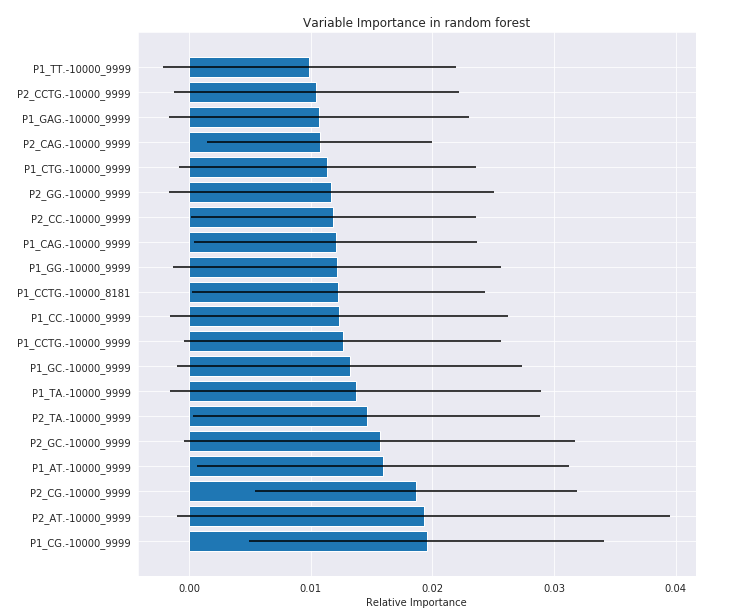
\includegraphics[scale=.4]{Images_Dextra/Var_imp_rf_prom_rates.png}
  \subfigure[2]{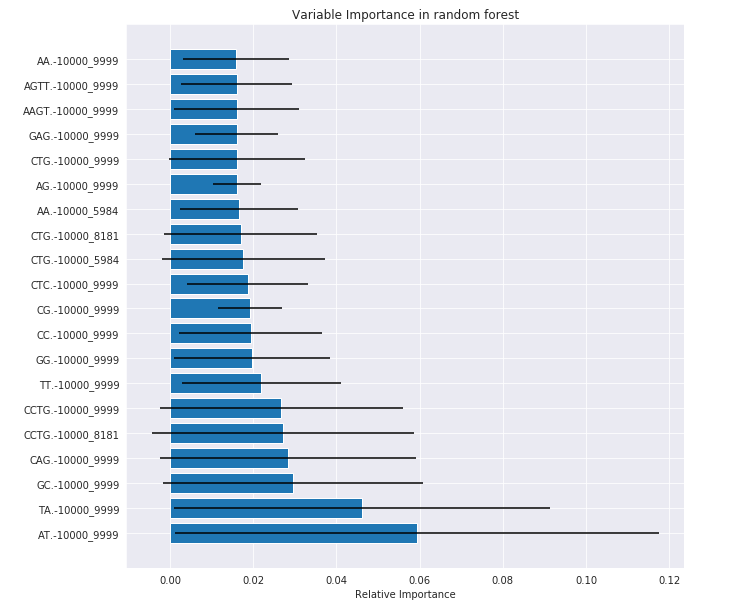
\includegraphics[scale=.4]{Images_Dextra/Var_imp_rf_diff_rates.png}\\
\end{center}
\caption{10 premières variables classées par importance par les \textit{Random Forests} entraînés.\\(1) : Taux pour chaque promoteur P1 et P2 de la paire. Nous voyons que lorsque la variable d'un promoteur P1 est sélectionnée, cette même variable chez P2 apparaît non loin dans le classement, confirmant leur combinaison par le modèle.\\(2) : Différence en valeur absolue des taux de P1 et P2. \\}
\label{fig:imp_rf}
\end{figure}

\begin{figure}[h]
\begin{center}
  \subfigure[1]{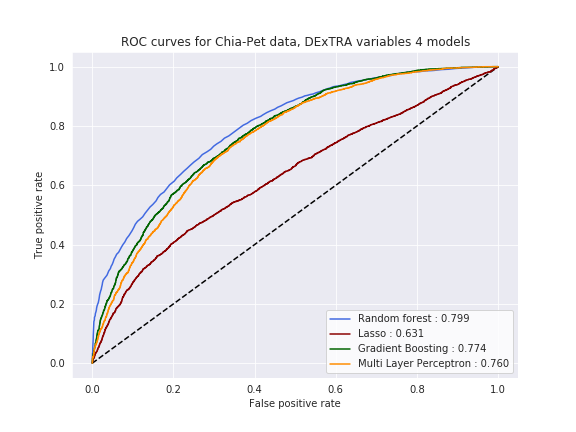
\includegraphics[scale=.5]{Images_Dextra/ROC_prom_rates.png}
  \subfigure[2]{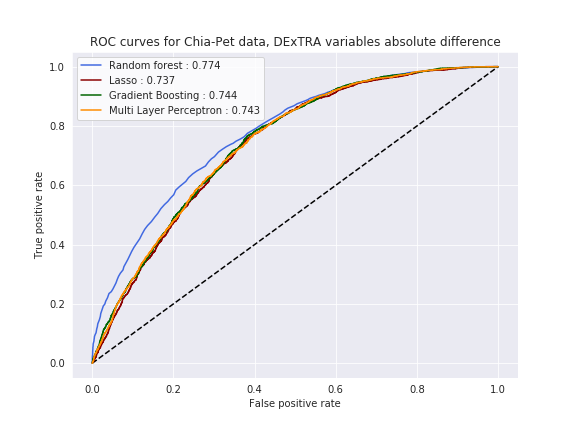
\includegraphics[scale=.5]{Images_Dextra/ROC_diff_rates.png}\\
\end{center}
\caption{Courbes ROC pour les configurations 1 et 2\\(1) : Taux pour chaque promoteur de la paire\\(2) : Différence en valeur absolue des deux taux}
\label{fig:aucs_dextra_configs}
\end{figure}

\end{document}


Consignes

UCBL
Le rapport doit faire entre 20 et 30 pages (hors annexes). Il peut être rédigé en français ou en anglais.

Le style à utiliser pour votre rapport est le style LNCS de Springer (exemple ). Vous trouverez dans cette archive un exemple LateX vous permettant de préparer au mieux votre rapport. Les templates LateX et Word sont aussi téléchargeables sur le site de Springer.

La qualité de la rédaction (orthographe, grammaire, tournures) et le soin général (respect du style LNCS, structure) apportés au document font partie intégrante des critères d'évaluation du rapport.

Les rapports sont à déposer sous forme d'un fichier PDF sur Easychair au plus tard selon les dates précisées ici.

INSA

Il vous est demandé de rédiger un texte scientifique ou technique, avec une introduction
qui situe le sujet, une présentation des matériels, méthodes ou modèles que vous avez utilisés, un
exposé des résultats obtenus, une discussion de ceux-ci, une conclusion et les perspectives
ouvertes par votre travail. Respectez ce format ! La bibliographie doit être présentée de manière
standard, en faisant apparaître le titre, le nom des auteurs et les références complètes des articles ou des ouvrages cités.

En préambule à ce rapport, vous commencerez par une courte présentation de la société ou
du laboratoire dans lequel vous avez effectué votre stage. L’objectif de cette partie est de vous
inciter à mieux connaître la structure d’accueil. Votre texte se terminera par un « rapport
d’étonnement » sur cette expérience professionnelle. Ce rapport d’étonnement, exprimant votre
ressenti quant à votre stage et son organisation, n’a pas nécessairement vocation à être relu par
votre tuteur de stage. Il peut donc être rendu sous forme séparée dudit rapport.

Le texte peut être rédigé en français ou en anglais.


Rapports de stage : limités à 30 pages au maximum (tout dépassement sera sanctionné).
Toutes les pages doivent être numérotées, y compris celles qui portent des tableaux ou des
figures. Les seules pages qui n’interviennent pas dans le total des 30 sont la page de titre, les
remerciements, le résumé, la bibliographie et les annexes.
Les soutenances ont lieu avant le jury de juillet ou de septembre selon la date de fin de stage.
Vous disposez de 20 minutes pour exposer votre travail ; cette présentation est suivie de 20
minutes de questions. La soutenance peut être publique ou à huis clos en cas de confidentialité.
Vous êtes responsable de l'organisation de cette soutenance, avec votre référent. Un
second enseignant INSA/UCBL doit être présent : à vous de le tr
ouver, avec l'aide éventuelle
du référent. Vous devez donc fixer à l'avance une date/heure de soutenance, au plus tard 4 jours
avant le jury de septembre pour avoir le temps de communiquer les notes.
Le rapport doit être rendu au moins 8 jours avant cette soutenance, à votre référent et
éventuellement au second enseignant, et déposé sur l’application. Vous devez également vous
assurer qu’il a bien reçu l’évaluation du tuteur de stage, au plus tard au moment de la
soutenance.


abstract : 

